%%%%%%%%%%%%%%%%%%%%%%%%%%%%%%%%%%%%%%%%%%%%%%%%%%%%%%%%%%%%%%%%%%%%%%%%%%%%%%%%
%%%%%%%%%%%%%%%%%%   Vorlage für eine Abschlussarbeit   %%%%%%%%%%%%%%%%%%%%%%%%
%%%%%%%%%%%%%%%%%%%%%%%%%%%%%%%%%%%%%%%%%%%%%%%%%%%%%%%%%%%%%%%%%%%%%%%%%%%%%%%%

% Erstellt von Maximilian Nöthe, <maximilian.noethe@tu-dortmund.de>
% ausgelegt für lualatex und Biblatex mit biber

% Kompilieren mit
% lualatex dateiname.tex
% biber dateiname.bcf
% lualatex dateiname.tex
% lualatex dateiname.tex
% oder einfach mit:
% make

\documentclass[
  tucolor,
  BCOR=12mm,     % 12mm binding corrections, adjust to fit your binding
  parskip=half,  % new paragraphs start with half line vertical space
  open=any,      % chapters start on both odd and even pages
  cleardoublepage=plain,  % no header/footer on blank pages
]{tudothesis}


% Warning, if another latex run is needed
\usepackage[aux]{rerunfilecheck}

% just list chapters and sections in the toc, not subsections or smaller
\setcounter{tocdepth}{1}

%------------------------------------------------------------------------------
%------------------------------ Sprache und Schrift: --------------------------
%------------------------------------------------------------------------------
\usepackage{fontspec}
\defaultfontfeatures{Ligatures=TeX}  % -- becomes en-dash etc.

% german language
\usepackage{polyglossia}
\setdefaultlanguage{german}

% for english abstract and english titles in the toc
\setotherlanguages{english}

% intelligent quotation marks, language and nesting sensitive
\usepackage[autostyle]{csquotes}

% microtypographical features, makes the text look nicer on the small scale
\usepackage{microtype}

%------------------------------------------------------------------------------
%------------------------ Für die Matheumgebung--------------------------------
%------------------------------------------------------------------------------

\usepackage{amsmath}
\usepackage{amssymb}
\usepackage{mathtools}
% Enable Unicode-Math and follow the ISO-Standards for typesetting math
\usepackage[
  math-style=ISO,
  bold-style=ISO,
  sans-style=italic,
  nabla=upright,
  partial=upright,
]{unicode-math}
\setmathfont{Latin Modern Math}

% nice, small fracs for the text with \sfrac{}{}
\usepackage{xfrac}



%------------------------------------------------------------------------------
%---------------------------- Numbers and Units -------------------------------
%------------------------------------------------------------------------------

\usepackage[
  locale=DE,
  separate-uncertainty=true,
  per-mode=symbol-or-fraction,
]{siunitx}
\sisetup{math-micro=\text{µ},text-micro=µ}

%------------------------------------------------------------------------------
%-------------------------------- tables  -------------------------------------
%------------------------------------------------------------------------------

\usepackage{booktabs}       % stellt \toprule, \midrule, \bottomrule
\usepackage{longtable}

%------------------------------------------------------------------------------
%-------------------------------- graphics -------------------------------------
%------------------------------------------------------------------------------

\usepackage{graphicx}
\usepackage{grffile}
\usepackage{subcaption}

% allow figures to be placed in the running text by default:
\usepackage{scrhack}
\usepackage{float}
\floatplacement{figure}{htbp}
\floatplacement{table}{htbp}

% keep figures and tables in the section
\usepackage[section, below]{placeins}


%------------------------------------------------------------------------------
%---------------------- customize list environments ---------------------------
%------------------------------------------------------------------------------

\usepackage{enumitem}

%------------------------------------------------------------------------------
%------------------------------ Bibliographie ---------------------------------
%------------------------------------------------------------------------------

% \usepackage[
%   backend=biber,   % use modern biber backend
%   autolang=hyphen, % load hyphenation rules for if language of bibentry is not
%                    % german, has to be loaded with \setotherlanguages
%                    % in the references.bib use langid={en} for english sources
% ]{biblatex}
% \addbibresource{references.bib}  % die Bibliographie einbinden
% \DefineBibliographyStrings{german}{andothers = {{et\,al\adddot}}}

\usepackage[
  style=numeric-comp,
  backend=biber,   % use modern biber backend
  autolang=hyphen, % load hyphenation rules for if language of bibentry is not
  sorting=none,   % german, has to be loaded with \setotherlanguages
  mcite=true,         % in the references.bib use langid={en} for english sources
]{biblatex}
%\addcontentsline{toc}{section}{Literaturverzeichnis}
\usepackage{atlasbiblatex}
\addbibresource{references.bib}
 % die Bibliographie einbinden
\DefineBibliographyStrings{german}{andothers = {{et\,al\adddot}}}


%------------------------------------------------------------------------------
%------------------------------ Sonstiges: ------------------------------------
%------------------------------------------------------------------------------

\usepackage[pdfusetitle,unicode,linkbordercolor=tugreen]{hyperref}
\usepackage{bookmark}
\usepackage[shortcuts]{extdash}
\usepackage{slashed}
\usepackage{tikz}
\usepackage[compat=1.0.0]{tikz-feynman}
\usepackage{icomma}
\usepackage{cancel}
\usepackage{multicol}
\newcommand{\uproman}[1]{\uppercase\expandafter{\romannumeral#1}}

%------------------------------------------------------------------------------
%-------------------------    Angaben zur Arbeit   ----------------------------
%------------------------------------------------------------------------------

\author{Janina Nicolini}
\title{Kombination und EFT-Interpretation von Messungen des \texorpdfstring {$t\bar{t}\gamma$}{math} Produktionswirkungsquerschnitts in Proton-Proton-Kollisionen}
\date{2018}
\birthplace{Aachen}
\chair{Lehrstuhl für Experimentelle Physik IV}
\division{Fakultät Physik}
\thesisclass{Bachelor of Science}
\submissiondate{31. Juli 2018}
\firstcorrector{Prof.~Dr.~Kevin Kröninger}
\secondcorrector{Dr.~Johannes Albrecht}

% tu logo on top of the titlepage
\titlehead{
\includegraphics[height=1.5cm]{logos/tu-logo.pdf}}

\begin{document}
\frontmatter
\maketitle

% Gutachterseite
\makecorrectorpage

% hier beginnt der Vorspann, nummeriert in römischen Zahlen
\thispagestyle{plain}
\section*{Kurzfassung}
Das Ziel dieser Arbeit ist die Kombination zweier Messungen des Produktionswirkungsquerschnitts für $t\bar{t}\gamma$-Ereignisse von ATLAS~\cite{Aaboud:2017era} und CMS~\cite{Sirunyan:2017iyh} mit Hilfe des frameworks EFTfitter\cite{Castro:2016jjv}. Dafür werden Ereignisse betrachtet, bei denen in Gluonfusion ein $t\bar{t}$-Paar entsteht und an einem Top-Quark ein Photon abgestrahlt wird.
Da die Messungen in unterschiedlichen Phasenräumen erfolgt sind, wird zunächst der Faktor zur Vereinheitlichung beider Phasenräume zu $f\approx 3$ bestimmt. Damit lässt sich die CMS-Messung in den ATLAS-Phasenraum extrapolieren. Die anschließende unkorrelierte Kombination ergibt einen Wirkungsquerschnitt von $\sigma_{\text{Kombi}} = 150 \pm 18~ \si{\femto\barn}$. Bei einer anschließenden Korrelationsstudie wird festgestellt, dass der kombinierte Wirkungsquerschnitt stark von der angenommenen Korrelation zwischen der ATLAS- und der CMS-Messung abhängt. Daher muss die Korrelation zunächst bestimmt werden. Aus den daraus folgenden Ergebnissen werden Einschränkungen für die
Wilson-Koeffizienten der beteiligten Operatoren einer effektiven Feldtheorie bestimmt. Die anschließende Untersuchung der Wilson-Koeffizienten $C_{tG}$, $C_{tW}$ und $C_{tB}$ ergibt, dass diese alle innerhalb des $1\sigma$-Intervalls mit Null verträglich sind.

\tableofcontents

\mainmatter
% Hier beginnt der Inhalt mit Seite 1 in arabischen Ziffern
\chapter{Einleitung}
Im Rahmen dieser Arbeit erfolgt eine Kombination und Interpretation des $t\bar{t}\gamma$-Produktionswirkungsquerschnitts von einer ATLAS-~\cite{Aaboud:2017era} und CMS-Messung~\cite{Sirunyan:2017iyh} im Rahmen von effektiven Feldtheorien (EFT). Dabei handelt es sich um eine Untersuchung im Hinblick auf Physik jenseits des Standardmodells (engl. \textit{beyond-the-standard-model}, BSM). Effektive Feldtheorien bieten dafür eine gute Grundlage, da sie es ermöglichen eine modellunabhängige Beschreibung neuer Phänomene zu liefern, ohne diese einzuschränken. Zudem können Energieskalen mit einbezogen werden, die mit heutigen Beschleunigern nicht zu erreichen sind. Eine Möglichkeit dies umzusetzen ist mit Hilfe von EFT-Operatoren, deren Kopplungsstärke an Standardmodell-Teilchen mit Wilson-Koeffizienten beschrieben werden kann. Es werden $t\bar{t}\gamma$-Ereigniss untersucht, da verschiedene Faktoren wie die große Top-Masse $m_t$ dafür sprechen, dass es besonders stark an BSM-Physik koppelt. Beide Messungen erfolgten dabei über Lepton+Jets-Endzustände.\\
Ziel dieser Arbeit ist es mit dem EFT\textit{fitter}~\cite{Castro:2016jjv} Einschränkungen für die Wilson-Koeffizienten, auf die bei der Produktion von $t\bar{t}\gamma$-Ereignissen beteiligten Operatoren zu finden. Da mit einer steigenden Anzahl an Messungen diese Einschränkungen genauer werden, werden die beiden Messungen von ATLAS und CMS mit dem EFT\textit{fitter} kombiniert.
Um eine Kombination der beiden Messungen überhaupt zu ermöglichen, muss zunächst eine Phasenraumstudie durchgeführt werden. Dies lässt sich darauf zurückführen, dass die gemessenen Phasenräume nicht übereinstimmen und deshalb vereinheitlicht werden müssen. Dies geschieht mit Hilfe von MadGraph5~\cite{Alwall:2014hca}.\\
Im Anschluss an diese Angleichung der Phasenräume kann die Kombination der Messungen erfolgen; dies geschieht mit dem EFT\textit{fitter}. Eine erste Kombination erfolgt unter der Annahme, dass die Unsicherheiten der Messungen nicht korreliert sind. Im Anschluss erfolgt eine Korrelationsstudie, um zu untersuchen, ob eine Korrelation einen Einfluss auf das Ergebnis der Kombination hat. Da CMS bei der Messungen explizit zwischen den Endzuständen mit einem Elektron-Lepton und einem Myon-Lepton unterscheidet, wird sowohl die Korrelation der beiden CMS-Messungen untereinander, als auch zwischen diesen und der ATLAS-Messung untersucht.\\
Zur Bestimmung der Wilson-Koeffizienten wird zu Beginn ein Modell für diese mit MadGraph5 bestimmt und im Anschluss im EFTfitter implementiert. Es dient dazu, den Einfluss der Wilson-Koeffizienten auf das Messergebnis zu implementieren. Durch den Vergleich des Modells mit den Messungen ergeben sich die Grenzen für die beteiligten Wilson-Koeffizienten.

\chapter{Quantenfeldtheorien zur Beschreibung der Teilchenphysik}
\section{Das Standardmodell der Teilchenphysik}
Das Standardmodell (SM) der Teilchenphysik ist eine Sammlung aus Quantenfeldtheorien und Parametern, die eine Beschreibung der bisher bekannten Elementarteilchen und Wechselwirkungen ermöglicht. Diese Elementarteilchen werden anhand ihrer Quantenzahlen wie Spin, Ladung und Masse klassifiziert.
Es wird zwischen den Fermionen mit einem halbzaligen Spin und den Eichbosonen mit einem ganzzahligen Spin, sowie dem Higgs-Boson mit Spin $0$ unterschieden. Die Fermionen sind die Bausteine der Materie und werden wiederum in Quarks und Leptonen unterschieden. Diese setzen sich jeweils aus drei Generationen, die jeweils aus einem $\text{SU}(2)$ Dublett bestehen, zusammen.\\
Die elementaren Wechselwirkungen werden durch die Eichbosonen vermittelt. Es wird zwischen der durch das Photon $\gamma$ vermittelteten elektromagnetischen Wechselwirkung, der durch die $W^{\pm}$ und $Z^0$ Bosonen vermittelten schwachen Wechselwirkung und der starken Wechselwirkung unterschieden. Letztere wird durch die acht Gluonen $g$ übertragen, die an die Farbladung koppeln.\\
\begin{figure}[H]
  \centering
  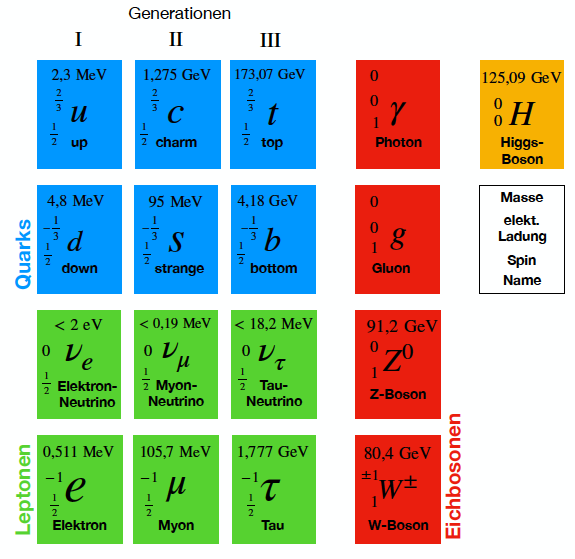
\includegraphics[width=0.6\textwidth]{Plots/SM.png}
  \caption{Schematische Darstellung der Elementarteilchen des SM\cite{Patrignani:2016xqp}.}
\end{figure}
Die Eichsymmetrie $SU(3)_\text{C} \times SU(2)_\text{L} \times U(1)_\text{Y}$ beschreibt diese Wechselwirkungen vor der Symmetriebrechung. Mit dem 2012 entdeckten, skalaren Higgs-Boson \cite{ Aad:2012tfa}\cite{Chatrchyan:2012xdj} kann das heutzutage bekannte SM durch den Lagrangian:
\begin{equation}
  \mathscr{L}_{SM} = - \frac{1}{4}F_{\mu\nu}F^{\mu\nu} + i \overline{\psi}\slashed{D}\psi + \psi_i Y_{ij} \psi_j \Phi + h.c. + |D_{\mu}\Phi|^2 - V(\Phi)
  \label{eqn:LSM}
\end{equation}
beschrieben werden. Der erste Term der Gleichung \eqref{eqn:LSM} beschreibt die kinetische Energie der Eichbosonen $\gamma$, $W^{\pm}$, $Z^0$ und $g$.
Hierbei treten Terme auf, die die Selbstkopplung der Gluonen beschreiben. Der zweite Term beschreibt die kinetische Energie der Fermionen und liefert damit eine Erklärung für die elementaren Wechselwirkungen mit den Eichfeldern.
Durch den Term $\psi_i Y_{ij} \psi_j \Phi + h.c.$ wird die Yukawa Wechselwirkung der Fermionen mit dem Higgsfeld dargestellt.
Dadurch lassen sich die Fermionenmassen und die Kopplung an das Higgs-Boson erklären.
Die kinetische Energie des Higgs-Bosons und damit dessen
Wechselwirkung mit den Eichfeldern wird durch den Term $|D_{\mu}\Phi|^2$ beschrieben. Obwohl Eichbosonen im Allgemeinen masselos sind, tragen das $W^{\pm}$ und $Z^0$ trotzdem eine Masse. Diese wird bei der spontanen Symmetriebrechung der Vereinheitlichung der QED und der schwachen Wechselwirkung $SU(2)_\text{L} \times U(1)_\text{Y}$, die durch den Higgs-Mechanismus verursacht wird, induziert. Der letzte Teil der Gleichung ist das Higgspotential. Dieses beinhaltet den Massenterm des Higgs-Bosons und beschreibt die Selbstkopplung des Higgs.

\section{Effektive Feldtheorie zur Erweiterung des Standardmodells}
Trotz der präzisen Beschreibung der bis heute entdeckten Teilchen und Wechselwirkungen gilt das SM als unvollständig. Es liefert beispielsweise keine Erklärung für die dunkle Materie, die aufgrund der abweichenden Rotationsgeschwindigkeit von Galaxien postuliert wurde \cite{Bertone:2016nfn}. Physikalische Theorien, die Effekte beschreiben, die über das SM hinausgehen, werden allgemein als Physik jenseits des SM (engl. \textit{beyond-the-standard-model}, BSM) bezeichnet. Da bis heute keine neuen Elementarteilchen bei der direkten Suche gemessen wurden, wird angenommen, dass diese zu schwer für die direkte Produktion an den heutigen Beschleunigern sind. Dies lässt vermuten, dass die Energieskala $\symup{\Lambda}$ der BSM-Physik, die des Standardmodells überschreitet. Trotz der aktuell nicht möglichen direkten Produktion könnten die Auswirkungen dieser neuen Teilchen auf andere Prozesse durch neue Effekte beobachtbar sein. Eine geeignete theoretische Beschreibung für diese Phänomene sind effektive Feldtheorien (EFT). Diese sind modellunabhängig und ermöglichen dadurch eine Beschreibung ohne einschränkende Annahmen für neue Wechselwirkungen. Ein sehr bekanntes Beispiel für eine EFT ist Fermis Erklärung des $\beta$-Zerfalls, der sich später mit der schwachen Wechselwirkung erklären ließ\cite{Fermi1934}.\\
Existiert ein neues Teilchen $X$, das leicht genug ist um es direkt zu produzieren, wird die Wechselwirkung mit anderen Teilchen durch den Propagator $\frac{1}{p^2 -m_X^2}$ beschrieben. Wenn dieses Teilchen jedoch zu schwer ist für die direkte Produktion, kann nur die indirekte Auswirkung auf die an der Wechselwirkung beteiligten Teilchen beschrieben werden. In diesem Fall lässt sich der Propagator um $\frac{p^2}{m_X^2}$ entwickeln, sodass er sich zu:
\begin{align}
    \frac{1}{p^2 -m_X^2} = -\frac{1}{m_X^2}\left[ 1 + \frac{p^2}{m_X^2} + \mathcal{O}\left(\frac{p^4}{m_X^4}\right)\right]
\end{align}
ergibt. Dies ermöglicht eine Parametrisierung der Auswirkung neuer Teilchen mit effektiven Operatoren.
Mit diesem Prinzip lassen sich effektive Feldtheorien ebenfalls mit einem Lagrangian beschreiben, der eine Parametrisierung von neuen Teilchen und eventuellen Wechselwirkungen ermöglicht. Die EFT-Operatoren tragen eine höhere Massendimension als die SM-Massendimension vier. Dabei ist zu beachten, dass die Auswirkungen der neuen Operatoren auf messbare Prozesse mit dem Inversen der Energieskala $\frac{1}{\Lambda^{d-4}}$ unterdrückt werden. Somit sinkt mit steigender Ordnung der Einfluss der Operatoren und damit die Wahrscheinlichkeit bei niedrigen Energien die Auswirkungen der entsprechenden Operatoren zu beobachten.\\
Der EFT-Lagrangian ist wie folgt definiert:
\begin{equation}
  \mathscr{L}_{EFT} = \sum_{d,i} \frac{1}{\Lambda^{d-4}} C_i O_i^{(d)}.
\end{equation}
Hierbei beschreiben die $O_i$ neue Operatoren höherer Ordnung und die $C_i$, die sogenannten Wilson-Koeffizienten, die individuellen Stärken dieser. Terme mit Massendimension $5$ entsprechen der Einführung von Majorana Massentermen. Diese sind jedoch für die Physik am Large Hadron Collider (LHC) uninteressant, da kein eichinvarianter Operator definiert werden kann, bei dem SM Quarks beteiligt sind. Somit können im Bereich der Top-Quark-Physik keine Effekte von Operatoren mit Massendimension fünf gemessen werden. Bei der Massendimension sechs ergeben sich hingegen insgesamt $59$ effektive Operatoren \cite{Grzadkowski:2010es}, von denen $15$\cite{Zhang:2014rja} an das
Feld des Top-Quarks koppeln.\\
Für die Operatoren mit der Massendimension sechs lässt sich ein Lagrangian durch:
\begin{equation}
  \mathscr{L}_{EFT, 6} = \mathscr{L}_{SM} + \mathscr{L}_{dim6} = \mathscr{L}_{SM} + \frac{1}{\Lambda^{2}} C_i O_i^{(6)}
\end{equation}
formulieren. Da der Lagrangian $\mathscr{L}_{EFT, 6}$ ebenfalls die Eichsymmetrie des SM erfüllen muss, geht er im Grenzfall in das Standardmodell über, sodass die Wilson-Koeffizienten in diesem Fall alle gleich 0 sind.

\section{Das Top Quark im Zusammenhang mit effektiver Feldtheorie}
\label{top}
Das Top Quark trägt Spin $\frac{\hbar}{2}$ und neben der elektrischen Ladung von $\frac{2}{3}$ der
Elementarladung $e$ auch eine Farbladung. Es nimmt wie alle Quarks an den drei fundamentalen Wechselwirkungen
teil. Durch seine hohe Masse $m_t = \SI{173.34(76)}{\giga\electronvolt}$~\cite{ATLAS:2014wva}, der höchsten eines
Elementarteilchens im SM, besitzt es nur eine sehr kurze Lebensdauer. Deshalb hadronisiert das
$t$-Quark nicht wie andere Quarks durch die starke Wechselwirkung, sondern zerfällt hauptsächlich über die schwache Wechselwirkung in ein $W$-Boson und ein $b$-Quark, wie in der CKM-Matrix an $|V_{tb}|^2 \approx 1$ zu erkennen ist.
Dieser Zerfall hat eine deutliche Signatur, die es ermöglicht eine sehr genaue Bestimmung der Quantenzahlen des Top-Quarks durchzuführen, sodass eine hohe Sensitivität in Bezug auf mögliche Abweichungen durch BSM-Physik erreicht wird.
Der Grundgedanke bei der Suche nach neuen physikalischen Effekten ist, dass neue Teilchen auf Grund ihrer hohen Masse besonders stark an das Higgs-Boson koppeln. Da das $t$-Quark das einzige SM-Fermion ist mit einer Yukawa-Kopplung von ungefähr $1$, wird davon ausgegangen, dass es ebenfalls besonders stark an die neuen Teilchen koppelt. Dies motiviert eine genaue Untersuchung des Top-Sektors in Bezug auf BSM-Physik.\\
Ein Prozess bei dem möglicherweise BSM-Physik-Effekte beitragen, ist die Abstrahlung eines Photons an einem $t$-Quark. Dies kann mit einem effektiven Vertex, wie in Abbildung~\ref{fig:eftVertex} dargestellt, beschrieben werden. Die Betrachtung dieses Vertex ist dadurch motiviert, dass er ebenfalls in einem Schleifenprozess in der $b$-Physik, wie in Abbildung~\ref{fig:bsa} dargestellt, vorkommt. Dort wurde bereits nach Auswirkungen von BSM-Physik gesucht. Daher ist es interessant zu untersuchen, ob die beteiligten Wilson-Koeffizienten des Vertex in der Top-Physik zu den gleichen Eingrenzungen führen.\\
Grundlage dieser Arbeit ist der $t\bar{t}\gamma$ Produktionswirkungsquerschnitt, der zum Beispiel in Prozessen wie in Abbildung~\ref{fig:tta} verdeutlicht, vorkommt. Hierbei kommt es zu Wechselwirkungen, die durch die drei BSM-Operatoren $O_{tB}, O_{tW}$ und $O_{tG}$ beschrieben werden können\cite{Bylund:2016phk}.
\begin{figure}
  \centering
  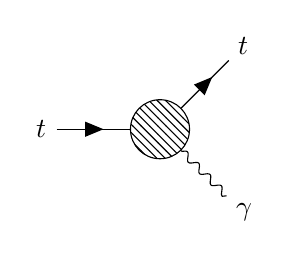
\begin{tikzpicture}
    \begin{feynman}
      \vertex (q1) {\(t\)};
      \vertex [right=1.5cm of q1, blob] (q2) {};
      \vertex [below right=1.5cm of q2] (q3) {\(\gamma\)};
      \vertex [above right=1.5cm of q2] (q4) {\(t\)};

      \diagram* {
        (q1) -- [fermion] (q2) -- [fermion] (q4),
        (q2) -- [boson] (q3),
      };
    \end{feynman}
  \end{tikzpicture}
  \caption{Darstellung des effektiven Vertex bei der Abstrahlung eines Photons $\gamma$ am $t$-Quark.}
  \label{fig:eftVertex}
\end{figure}
Dabei wird $O_{tG}$ betrachtet, weil das $t$-Quark aus Gluonfusion entsteht und $O_{tB}$ und $O_{tW}$ wegen der Photonabstrahlung.
\begin{align}
   O_{tW} &= y_t g_w \left(\bar{Q}\sigma^{\mu\nu}\tau^{I} t \right) \tilde{\varphi} W^{I}_{\mu\nu}\\
   O_{tB} &= y_t g_Y \left(\bar{Q}\sigma^{\mu\nu} t \right) \tilde{\varphi} B_{\mu\nu}\\
   O_{tG} &= y_t g_s \left(\bar{Q}\sigma^{\mu\nu}T^A t\right)\tilde{\varphi}~ G^{A}_{\mu\nu}
\end{align}
Hierbei steht $Q$ für das linkshändige Quarkdublett der dritten Generation, $\varphi$ für das Higgsfeld und $g_w$, $g_Y$ und $g_s$ sind die SM Eichkopplungskonstanten. Die Yukawa Kopplung des Top-Quarks wird mit $Y_t = \frac{\sqrt{2}m_t}{v}$ beschrieben, bei der $v = \SI{246}{\giga\electronvolt}$ der Higgsvakuumserwatungswert ist.\\
Dies motiviert die Wilson-Koeffizienten dieser Operatoren hier näher zu untersuchen. Wenn ein Vergleich dieser Operatoren mit denen, die bei dem Prozess \ref{fig:bsa} beteiligt sind, angestrebt wird, muss beachtet werden, dass sich die Benennung unterscheidet und die Bestimmung auf unterschiedlichen Energieskalen erfolgt.

\begin{figure}
  %\centering
    \begin{subfigure}[b]{0.45\textwidth}
      \centering
      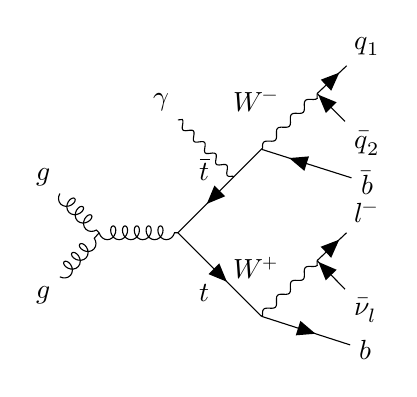
\begin{tikzpicture}
        \begin{feynman}
            \vertex (a) {\(g\)};
            \vertex [below=1.5cm of a] (b) {\(g\)};
            \vertex [below right=1cm of a] (a1);
            \vertex [right=1cm of a1] (a2);
            \vertex [above right=1cm of a2] (a4);
            \vertex [above left= 1cm of a4] (a5) {\(\gamma\)};
            \vertex [above right=0.5cm of a4] (a3);
            \vertex [above right=1cm of a3] (c);
            \vertex [above right=0.5cm of c] (c1) {\(q_{1}\)};
            \vertex [below right=0.5cm of c] (c2) {\(\bar{q}_2\)};
            \vertex [below=0.5cm of c2] (d) {\(\bar{b}\)};
            \vertex [below right=0.5cm of a2] (b1);
            \vertex [below right=1cm of b1] (b2);
            \vertex [above right=1cm of b2] (b3);
            \vertex [above right=0.5cm of b3] (d1) {\(l^{-}\)};
            \vertex [below right=0.5cm of b3] (d2) {\(\bar{\nu}_l\)};
            \vertex [below=0.5cm of d2] (d3) {\(b\)};
            \diagram* {
              (a) -- [gluon] (a1),
              (b) -- [gluon] (a1) -- [gluon] (a2),
              (a2) -- [anti fermion, edge label=\(\overline t\)] (a3) -- [anti fermion] (d),
              (a3) -- [boson, edge label=\(W^{-}\)] (c) -- [fermion] (c1),
              (c) -- [anti fermion] (c2),
              (a2) -- [fermion, edge label'=\(t\)] (b2),
              (b2) -- [boson, edge label=\(W^{+}\)] (b3) -- [fermion] (d1),
              (b3) -- [anti fermion] (d2),
              (b2) -- [fermion] (d3),
              (a4) -- [boson] (a5),
            };
        \end{feynman}
      \end{tikzpicture}
      \subcaption{Zerfall eines $t$-Quarks in ein $W$-Boson und ein $b$-Quark unter Abstrahlung eines Photons~$\gamma$.}
      \label{fig:tta}
    \end{subfigure}
    \hfill
    \begin{subfigure}[b]{0.45\textwidth}
      \centering
      \begin{tikzpicture}
        \begin{feynman}
          \vertex (a1) {\(b\)};
          \vertex[right=1.5cm of a1] (a2);
          \vertex[right=1cm of a2] (a3);
          \vertex[below=1cm of a3] (c2) {\(\gamma\)};
          \vertex[right=1cm of a3] (a4);
          \vertex[right=1.5cm of a4] (a5) {\(s\)};
          \diagram* {
          (a1) -- [fermion](a2),
          (a2) -- [fermion, edge label'=\(t\)] (a3),
          (a3) -- [boson] (c2);
          (a3) -- [fermion, edge label'=\(t\)] (a4),
          (a4) -- [fermion] (a5),
          (a4) -- [boson, out=90, in=90, looseness=2, edge label'=\(W^{-}\)] (a2)
          };
        \end{feynman}
      \end{tikzpicture}
      \subcaption{Zerfall eines $b$-Quarks in ein $s$-Quark unter Abstrahlung eines Photons~$\gamma$ im Loop.}
      \label{fig:bsa}
    \end{subfigure}
  \caption{Prozesse aus der Top-Quark- und der Bottom-Quark-Physik bei denen der effektive Vertex $t\bar{t}\gamma$ beteiligt ist.}
\label{fig:feynman}
\end{figure}

\chapter{Vereinheitlichung zweier Messungen des \texorpdfstring {$t\bar{t}\gamma$}{math} Produktionswirkungsquerschnitts mit dem EFTfitter}%
In diesem Kapitel erfolgt die Kombination der Messungen von ATLAS und CMS für den $t\bar{t}\gamma$ Produktionswirkungsquerschnitt bei einer Schwerpunktsenergie von $\sqrt{s} = \SI{8}{\tera\electronvolt}$. Da die Messungen in unterschiedlichen Phasenräumen erfolgt sind, wird vor der eigentlichen Kombination mit dem EFTfitter eine Phasenraumstudie durchgeführt, um die Phasenräume zu vereinheitlichen.

\section{\texorpdfstring {$t\bar{t}\gamma$}{math} Messungen von ATLAS und CMS}%
\label{kap:messung}
Die Messungen des Produktionswirkungsquerschnitts von ATLAS\cite{Aaboud:2017era} und CMS\cite{Sirunyan:2017iyh} sind beide bei einer Proton-Proton-Kollision bei einer Schwerpunktsernegie von $\sqrt{s}=\SI{8}{\tera\electronvolt}$ durchgeführt worden. Die Bestimmung des Wirkungsquerschnitts erfolgt über den semileptonischen Endzustand. Somit zerfällt eins der entstehenden $W$-Bosonen in ein Elektron oder Myon mit dem entsprechenden Neutrino und das andere $W$-Boson hadronisch. Ein möglicher Feynman-Graph für diesen Prozess ist in~\ref{fig:tta} dargestellt.\\
Obwohl ATLAS und CMS den gleichen Prozess betrachtet haben, unterscheiden sich die Messungen grundlegend durch den zu Grunde liegenden gemessenen Phasenraum. Die Wahl den gemessenen Phasenraum zu betrachten, hat den Vorteil, dass die Modellunabhängigkeit maximiert wird und die Extrapolation in den experimentell nicht messbaren Phasenraum minimiert wird. Die von ATLAS und CMS verwendeten Schnitte für ihren gemessenen Phasenraum sind in Tabelle \ref{tab:cut}
aufgeführt.\\
%
 \begin{table}[H]
     \centering
    \begin{tabular}{c|l|l}
      Objekte & ATLAS & CMS \\
      \hline
      \textbf{Photon} & $p_T > \SI{15}{\giga\electronvolt}\quad |\eta| < 2,37$ & $p_T > \SI{25}{\giga\electronvolt}\quad |\eta| < 1,44$\\
      Leptonen & $p_T > \SI{25}{\giga\electronvolt}\quad |\eta| < 2,5$ & $\text{e}:\: p_T > \SI{35}{\giga\electronvolt}\quad |\eta| < 2,5$ \\
      {} & {} & $\symup{\mu}:\: p_T > \SI{26}{\giga\electronvolt}\quad |\eta| < 2,5$\\
      Jets & $p_T > \SI{25}{\giga\electronvolt}\quad |\eta| < 2,5$ & $p_T > \SI{30}{\giga\electronvolt}\quad |\eta| < 2,4$\\
      b-Jets & $p_T > \SI{5}{\giga\electronvolt}$ &  \\
      Neutrino &  & $p_T^{miss} > \SI{20}{\giga\electronvolt}$
    \end{tabular}
    \caption{Verwendete Schnitte auf den gemessenen Phasenraum.}
    \label{tab:cut}
 \end{table}
Dabei fällt auf, dass die Schnitte für das Photon sich deutlich unterscheiden. So setzt ATLAS einen Transversalimpuls von $p_{T} > \SI{15}{\giga\electronvolt}$ voraus, wohingegen CMS mindestens $p_{T} > \SI{25}{\giga\electronvolt}$ einfordert. Außerdem wählt ATLAS eine Pseudorapidität von $|\eta| < 2,37$, während CMS $|\eta| < 1,44$ annimmt. Zudem setzt CMS einen durch das Neutrino fehlenden Transversalimpuls von $p_{T}^{miss} > \SI{20}{\giga\electronvolt}$ voraus.
ATLAS setzt zudem zwischen dem Photon und dem Lepton mindestens ein Abstand von $\symup{\Delta} R(\gamma, \text{l}) = 0,7$, zwischen dem Photon und dem Jet $\symup{\Delta} R(\gamma, \text{Jet}) = 0,5$ und zwischen dem $b$-Quark und dem Jet $\symup{\Delta} R(\text{b}, \text{Jet}) = 0,3$ vorraus.
Das CMS Papier umfasst keine weiteren Angaben zur Isolation der Objekte.\\
Die von ATLAS und CMS gemessenen Produktionswirkungsquerschnitte für $t\bar{t}\gamma$ ergeben sich zu:
\begin{align*}
  \sigma^{fid, \text{ATLAS}}_{t\bar{t}\gamma} &= 139 \pm 18~\text{(stat.$+$syst.)}~ \si{\femto\barn}\\
  \sigma^{fid, \text{CMS}}_{t\bar{t}\gamma, e} &= 138 \pm 45~\text{(stat.$+$syst.)}~ \si{\femto\barn}\\
  \sigma^{fid, \text{CMS}}_{t\bar{t}\gamma, \mu} &= 115 \pm 32~\text{(stat.$+$syst.)}~ \si{\femto\barn}.
\end{align*}
CMS unterscheidet dabei zwischen zwei Wirkungsquerschnitten, bei denen das Lepton im Endzustand einmal ein Elektron und einmel ein Myon ist.

\section{Kombinationen mit dem EFTfitter}
Der EFTfitter\cite{Castro:2016jjv} ist ein Programm, das es ermöglicht Studien zur BSM-Physik auf Grundlage von effektiven Feldtheorien durchzuführen. Er erlaubt Benutzern physikalische Modelle selbst zu implementieren und im
Zusammenhang der Wahrscheinlichkeitsrechnung nach Bayes zu testen. Zudem ist eine Kombination verschiedener Messungen möglich, ohne diese selbst durchgeführt zu haben.
Bei solchen Kombinationen ist die Breite der Wahrscheinlichkeitsverteilung und damit ihre Aussagekraft von der Anzahl der Messungen abhängig.
Die Bayessche Inferenz ermöglicht eine Anpassung des Modells an die Daten, sodass eine Wahrscheinlichkeitsverteilung für den gesuchten Parameter des Modells erhalten wird.\\
Die Grundlage für diese Berechnungen liefert der Satz von Bayes:
\begin{align}
  p(\lambda|x) = \frac{L(x|\lambda) \cdot \pi(\lambda)}{p(x)}.
\end{align}
Der gesuchte Parameter des Modells ist $\lambda$ und die verwendete Datenmenge wird in diesem Fall durch $x$ beschrieben. Die A-Prioriverteilung $\pi(\lambda)$ enthält Informationen über die zu untersuchende Variable $\lambda$. Dies können zum Beispiel physikalische Konstanten sein, die zum Implementieren des Modells benötigt werden.
Die Normierung $p(x)$ wird mit:
\begin{align}
  p(x) = \int d\lambda L(x|\lambda) \cdot \pi(\lambda)
\end{align}
berechnet. Die Likelihood $L(\vec{x}|\lambda)$ beschreibt die Wahrscheinlichkeitsverteilung der Daten $\vec{x}$. Die gesuchte Posteriorverteilung wird durch $p(\lambda|\vec{x})$ beschrieben. Diese beinhaltet neue Erkenntnisse über den Parameter $\lambda$, die aus den Daten gewonnen werden. Somit kann die anfängliche Erkenntnis über den Parameter $\lambda$ verbessert werden.\\
Werden für eine Kombination $n$ Messungen $x_i$ mit $(i= 1,...,n)$ und $N$ Observablen $y_i$ mit $(i= 1,...,N)$ betrachtet, kann die Likelihood als gaußförmig angenommen werden und wird mit:
\begin{align}
  -2 \ln{L(\mathbf{x}|\lambda)} = \sum^{n}_{i=1} \sum^{n}_{j=1} \left[\mathbf{x} - U\mathbf{y}\right]_{i} \mathcal{M}_{ij}^{-1} \left[\mathbf{x} - U\mathbf{y}\right]_{j}
  \label{eqn:like}
\end{align}
beschrieben. $U_{ij}$ ist das Matrixelement einer $n \times N$-Matrix $U$, welches eins ist, wenn $x_i$ die Messung zur Observable $y_i$ ist und ansonsten null. Da die Unsicherheiten der Messung $x_i$ korreliert sein können, beschreibt
\begin{align}
  \mathcal{M}_{ij} = \text{cov}[x_i, x_j] = \sum_{k=1}^{M} \text{cov}^{(k)}[x_i, x_j]
\end{align}
die Elemente der symmetrischen und positiv semidefiniten Kovarianzmatrix, bei der $M$ die Anzahl der verscheidenen Quellen an Unsicherheiten ist. Das mit dem EFTfitter berechnete Ergebnis wird ebenfalls bei der Verwendung der BLUE-Methode (\textit{best linear unbiased estimator})\cite{LYONS1988110} erhalten. Da diese einen Spezialfall des EFTfitter bildet und einer Minimierung der Likelihood \eqref{eqn:like} entspricht.

\section{Phasenraumstudie mit MadGraph5}
\label{phasencms}
Um eine Kombination der beiden Messungen des $t\bar{t}\gamma$ Wirkungsquerschnitts von CMS und ATLAS ermöglichen zu können, muss zuvor eine Phasenraumstudie durchgeführt werden. Da beide Messungen in unterschiedlichen Phasenräumen durchgeführt wurden, müssen sie zunächst vereinheitlicht werden.
Der Vergrößerung eines Phasenraums liegt ein linearer Zusammenhang zu Grunde, sodass als erste Approximation ein Faktor zwischen den beiden Phasenräumen bestimmt werden kann. Dazu können mit Hilfe des Monte Carlo Generators MadGraph5\cite{Alwall:2014hca} (MG) zunächst die beiden Produktionswirkungsquerschnitte für $t\bar{t}\gamma$ berechnet werden.
Anschließend werden diese beiden Werte durcheinader geteilt und der sich ergebene Faktor wird auf die CMS-Messung angewandt. Dadurch wird diese Messung in den Phasenraum der ATLAS Messung erweitert.\\
Zunächst einmal wird der semileptonische Zerfall des $t\bar{t}$-Quarkpaars unter Abstrahlung des Photons mit den expliziten Endzuständen in MG simuliert. Dazu wird das SM als Modell und das $\text{CTEQ}6\text{L}1$ PDF Set\cite{Paakkinen:2018zbs} zum Implementieren des Prozesses genutzt. Bei der Berechnung der semileptonischen Endzustände kann jedoch nur die führende Ordnung (\textit{leading-order}, LO) betrachtet werden. Für die Berechnung der Produktionswirkungsquerschnitte werden die in Kapitel \ref{kap:messung} angegebenen Schnitte genutzt. Da von der CMS-Kollaboration in dem Papier keine weiteren Aussagen über die Isolation der einzelnen Objekte gemacht werden, werden für diese Arbeit die gleichen Abstände wie bei ATLAS verwendet. Unter diesen Vorraussetzungen ergeben sich die Wirkungsquerschnitte aus der MG Simulation zu:
\begin{align}
  \sigma^{fid, \text{ATLAS}}_{\text{LO}} &= 146,5 \pm 0,095~ \si{\femto\barn}\\
  \sigma^{fid, \text{CMS}}_{\text{LO}} &= 49,29 \pm 0,034~ \si{\femto\barn}.
\end{align}
Auffällig ist dabei, dass der Wert von ATLAS $2,97$ mal so groß ist, wie der CMS Produktionswirkungsquerschnitt. Dies ist unerwartet, da beide Ergebnisse der Messungen sehr ähnlich sind und in den Papieren als vertäglich mit dem SM angesehen werden.
Beim Vegleich der Photon-Schnitte fällt jedoch auf, dass durch den höheren $p_T$-Schnitt von CMS bereits ungefähr $90000$ der anfänglichen $220000$ Ereignisse verloren gehen. Durch den Schnitt auf die Pseudorapidität entfallen ebenfalls nochmal etwa $45000$ Ereignisse. Dies entspricht etwa $\SI{60}{\percent}$ der anfänglichen Ereignisse, sodass der Faktor $3$ durchaus plausibel erscheint. Eine Veranschaulichung dieser Änderungen befindet sich in Abbildungildung \ref{fig:schnitte}.\\
\begin{figure}
    \begin{subfigure}[c]{0.5\textwidth}
      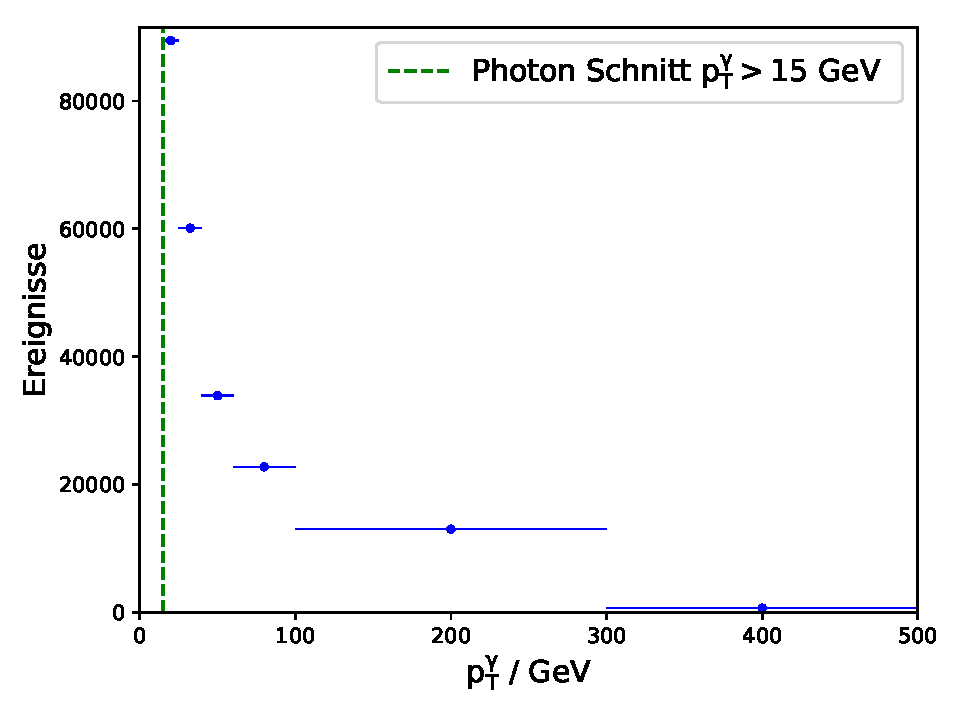
\includegraphics[width=\textwidth]{Plots/photon_pt_Atlas.pdf}
      \subcaption{ATLAS}
    \end{subfigure}
    \begin{subfigure}[c]{0.5\textwidth}
      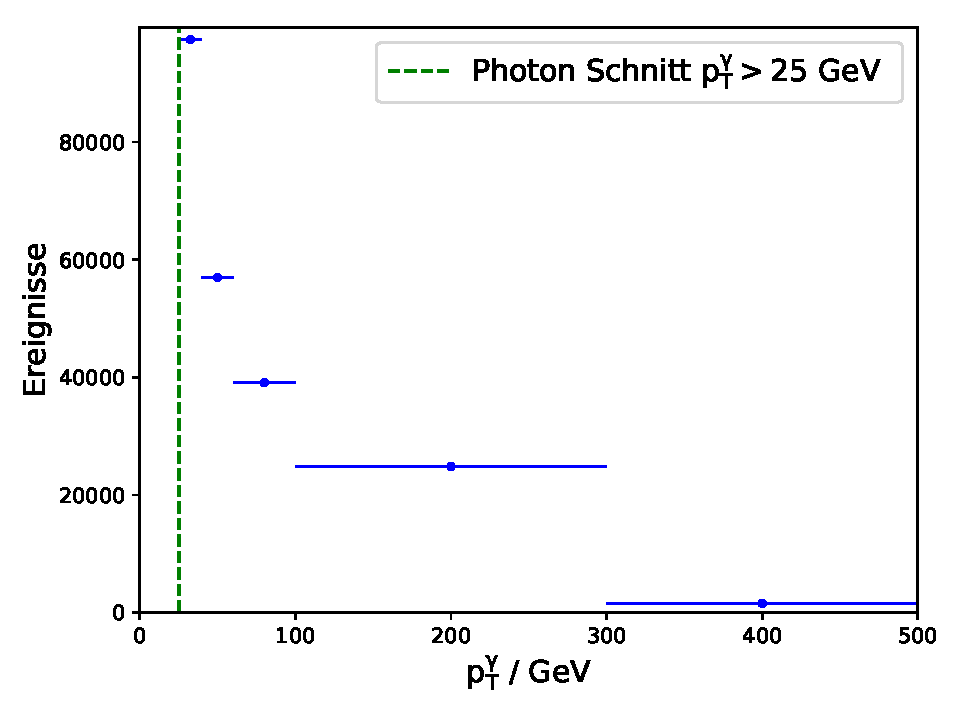
\includegraphics[width=\textwidth]{Plots/photon_pt_Cms.pdf}
      \subcaption{CMS}
    \end{subfigure}
    \begin{subfigure}[c]{0.5\textwidth}
      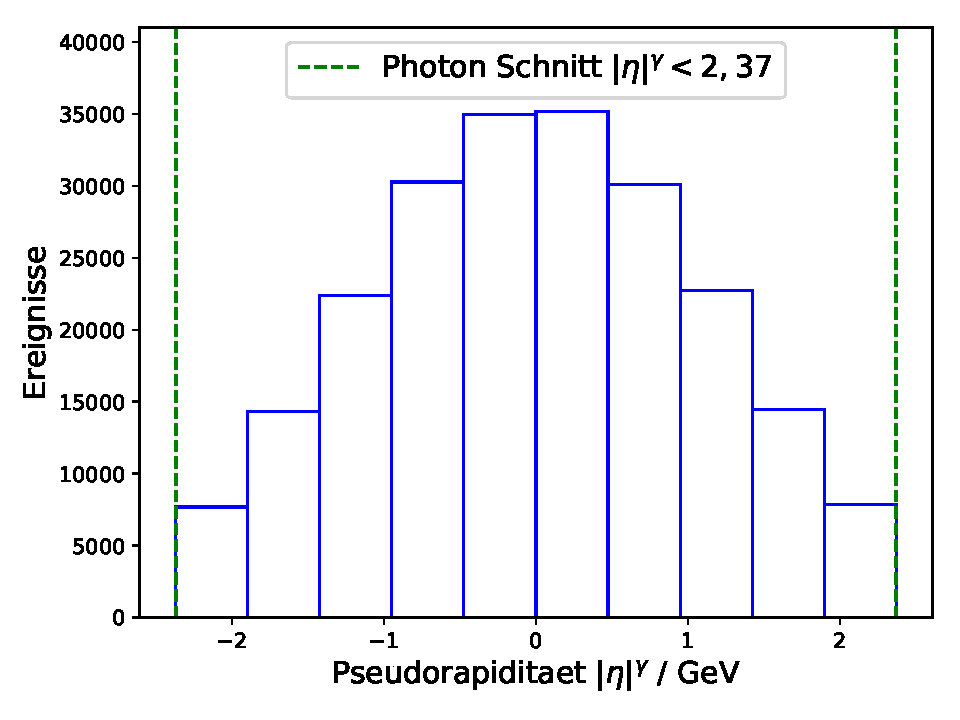
\includegraphics[width=\textwidth]{Plots/photon_eta_Atlas.pdf}
      \subcaption{ATLAS}
    \end{subfigure}
    \begin{subfigure}[c]{0.5\textwidth}
      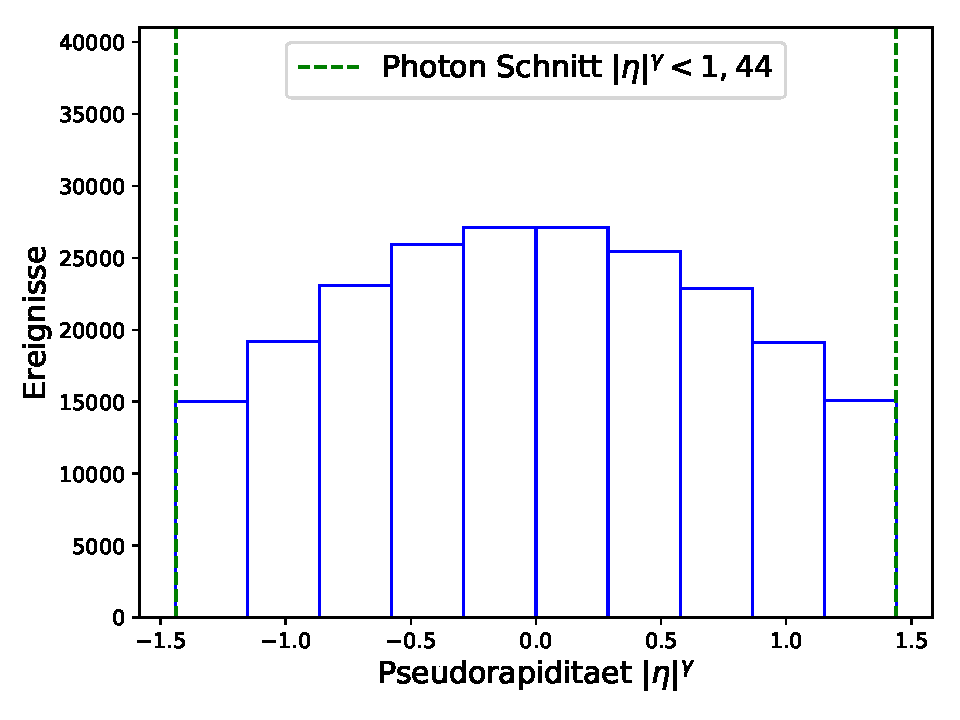
\includegraphics[width=\textwidth]{Plots/photon_eta_Cms.pdf}
      \subcaption{CMS}
    \end{subfigure}
    \caption{Verteilungen der Transversalimpulse und der Pseudorapidität der Photonen. Die grünen Linien representieren die von ATLAS und CMS verwendeten Schnitte. Die verwendeten Datensätze stammen aus Simmulationen mit MadGraph5.}
    \label{fig:schnitte}
\end{figure}
Um einen möglichst genauen Faktor zwischen den gemessenen Phasenräumen zu erhalten, wird eine Rechnung in der nächst-führenden Ordnung (\textit{next-to-leading-oder}, NLO) angestrebt. Dies ist bei MG für die expliziten Endzustände nicht möglich. Daher bietet es sich an, den Prozess $p~p~$\textrightarrow$~t~\bar{t}~\gamma$~ ohne diese, sowohl in LO als auch in NLO zu simulieren. Daraus kann im Anschluss ein $k$-Faktor als Näherung zwischen den beiden Ordnungen berechnet werden.\\
Damit ergeben sich folgende Wirkungsquerschnitte in der LO-Rechnung:
\begin{align}
  \sigma^{\text{ATLAS}}_{\text{LO}} &= 682,8 \pm 3,9~ \si{\femto\barn}\\
  \sigma^{\text{CMS}}_{\text{LO}} &= 361,6 \pm 1,5~ \si{\femto\barn}
\end{align}
und folgende Werte in der NLO-Rechnung:
\begin{align}
  \sigma^{\text{ATLAS}}_{\text{NLO}} &= 452,5 \pm 1,2~ \si{\femto\barn}\\
  \sigma^{\text{CMS}}_{\text{NLO}} &= 243,6 \pm 0,73~ \si{\femto\barn}.
\end{align}
Diese Wirkungsquerschnitte lassen sich durch Multiplizieren mit dem Verzweigungsverhältnis (\textit{branching ratio}, $\mathrm{BR}$) für den semileptonischen Zerfall in die, der expliziten Endzustände umrechnen. Das Verzweigungsverhältnis gibt die Wahrscheinlichkeit an, dass ein Zustand in einen bestimmten Endzustand zerfällt und liegt in diesem Fall bei $\mathrm{BR}=\SI{30}{\percent}$. Werden die Wirkungsquerschnitte nun mit der $\mathrm{BR}$ multipliziert und der NLO-Wert durch den der LO-Rechnung geteilt, ergibt sich folgender $k$-Faktor für ATLAS und CMS:
\begin{align}
  k_{\text{ATLAS}} &= \frac{0,3 \cdot 682,8~ \si{\femto\barn}}{0,3 \cdot 452,5~ \si{\femto\barn}} = 1,509\\
  k_{\text{CMS}} &= \frac{0,3 \cdot 361,6~ \si{\femto\barn}}{0,3 \cdot 243,6~ \si{\femto\barn}} = 1,484.
\end{align}
Auf Grund ihrer geringen Größe wurden die Fehler hier vernachlässigt. Unter Anwendung dieser $k$-Faktoren auf die zu Beginn bestimmten Produktionswirkungsquerschnitte ergibt sich der Phasenraumfaktor $f$ zwischen den gemessenen Phasenräumen von ATLAS und CMS zu:
\begin{align}
  f = \frac{1,509 \cdot 146,5~ \si{\femto\barn}}{1,484 \cdot 49,29~ \si{\femto\barn}} = 3,0221
\end{align}
Auch bei der Bestimmung mit einer Näherung für die NLO-Rechnung ergibt sich erneut ein Faktor der nahe an der drei liegt. Somit wird der CMS Phasenraum durch Multiplizieren mit einem Phasenraumfaktor von genau drei in den von ATLAS transformiert. Dabei ergeben sich die folgenden Produktionswirkungsquerschnitte:
\begin{align}
  \sigma^{fid(A), \text{CMS}}_{t\bar{t}\gamma, e} &= 410 \pm 140~ \si{\femto\barn}\\
  \sigma^{fid(A), \text{CMS}}_{t\bar{t}\gamma, \mu} &= 350 \pm 100~ \si{\femto\barn}.
\end{align}
Problematisch ist, dass bei dieser Rechnung über die Unsicherheit extrapoliert wird. Jedoch ist unklar, ob diese nicht nur im gemessenen CMS Phasenraum gültig sind. Diese Umrechnung wird trotzdem gewählt, da es sich lediglich um eine erste Näherung für die Vereinheitlichung der beiden Referenzphasenräume handelt. Dies bedarf weitergehender Studien durch eine aufwändigere Betrachtung der Unsicherheiten.
%
%
\chapter{Kombination der Messungen \texorpdfstring {$t\bar{t}\gamma$}{math}}
In diesem Kapitel wird die Vereinheitlichung der ATLAS und CMS Messungen unter der Verwendung des Ergebnisses aus dem Kapitel~\ref{phasencms} beschrieben. Hierbei ist zu beachten, dass die Kombination zuerst einmal unter der Annahme erfolgt, dass zwischen den drei Messergebnissen keine Korrelationen vorliegen. Um diese Annahme zu rechtfertigen, wird anschließend eine Korrelationsstudie für die Korrelation zwischen den beiden CMS Messungen durchgeführt.

\section{Gesamtkombination}
\label{kombi}
Wird eine unkorrelierte Kombination des angegebenen Produktionswirkungsquerschnitts von ATLAS und der in den gemessenen Phasenraum von ATLAS erweiterteten Messungen von CMS mit dem EFTfitter durchgeführt, ergibt sich der Wirkungsquerschnitt von $t\bar{t}\gamma$ zu:
\begin{align}
  \sigma_{\text{Kombi}} = 149,79 \pm 17,57~ \si{\femto\barn}.
\end{align}
Auffällig ist, dass das kombinierte Ergebnis sehr dicht an dem von ATLAS gemessenen Wert liegt.
Dies ist damit zu begründen, dass der EFTfitter eine Gewichtung der gegebenen Messungen anhand ihrer Unsicherheiten durchführt.
Durch die Extrapolation über die Unsicherheiten der CMS Messungen liegen diese in der selben Größenordnung wie die Nominalwerte, sodass diese Wirkungsquerschnitte bei der Berechnung der Kombination des EFTfitters nur sehr gering beitragen. Bei der Betrachtung der gaußförmigen Verteilungen um den gemessenen Produktionswirkungsquerschnitt in Abbildung~\ref{fig:gau} fällt auf, dass die Verteilungen für die CMS Messungen deutlich breiter sind und somit der Informationsgehalt für die ATLAS Messung höher ist. Dies erklärt die geringe Gewichtung der CMS Messungen durch den EFT-Fitter.\\
Dieses Ergebnis motiviert neben den Ergebnissen aus Kapitel~\ref{phasencms} ebenfalls eine genauere Betrachtung der Unsicherheiten und ihrer Gültigkeit in dem erweiterten Phasenraum. Zudem bietet es sich an, eine Korrelationsstudie durchzuführen, da für diese erste Kombination die Messungen als unkorreliert angenommen wurden.

\begin{figure}
  \centering
  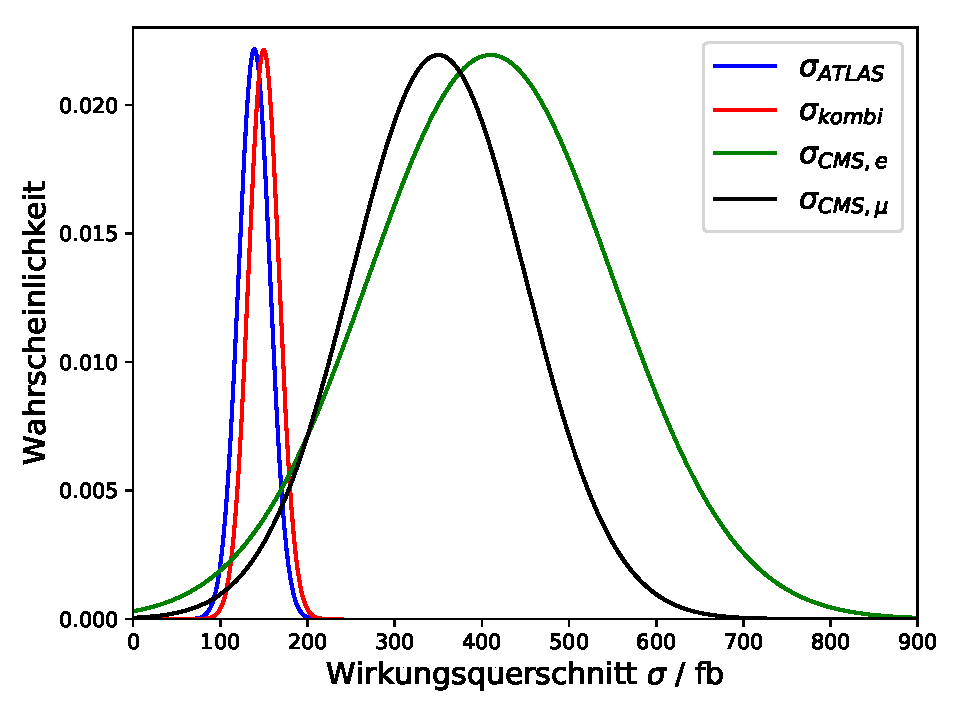
\includegraphics[width=0.8\textwidth]{Plots/gauss.pdf}
  \caption{Veranschaulichung der gaußverteilten Unsicherheiten um den Mittelwert der verschiedenen Messungen.}
  \label{fig:gau}
\end{figure}

\section{Korrelationsstudie}
Um eine unkorrelierte Kombination der drei Messungen zu rechtfertigen, wird eine Korrelationsstudie durchgeführt. Dabei wird zunächst nur eine Korrelation zwischen den beiden CMS Messungen untersucht. Hierfür werden die Ergebnisse aus Kapitel~\ref{phasencms} verwendet. Die verwendete Korrelationsmatrix ist symmetrisch, positiv semidefinit und hat die Form:
\begin{align}
  \text{Corr}_{\sigma,\text{CMS}}\,=\begin{pmatrix}
  1 & \rho_{e, \mu}\\
  \rho_{\mu, e} & 1
  \end{pmatrix}.
  \label{eqn:matrix1}
\end{align}
Aus diesem Grund wird für eine erste Betrachtung $\rho_{e, \mu}= \rho_{\mu, e}$ im Bereich $[-0,9~,~0,9]$ in $0,1$ Schritten variiert. Eine Kombination der beiden semileptonischen Produktionswirkungsquerschnitte von CMS unter Verwendung der Korrelationsmatrix $\text{Corr}_{\sigma,\text{CMS}}$ ist in Abbildung~\ref{fig:corrcms} dargestellt. Dabei lässt sich ein nahezu linearer Verlauf erkennen, der lediglich im Bereich hoher positiver Korrelationen abweicht. Da keine Effekte zu erkennen sind, scheint die Annahme, dass die Messungen nicht korreliert sind gerechtfertigt zu sein. Die großen Fehlerbalken lassen sich auf die großen Unsicherheiten der beiden Messungen zurückführen. Zudem wachsen sie bei einer positiven Korrelation weiter an, da die Messungen beide stärker gewichtet werden. Bei der negativen Korrelation wird hingegen die Gewichtung der zweiten Messung immer geringer, sodass bei einer großen, negativen Korrelationen eine Messung und damit ihre Unsicherheit sehr gering beiträgt.\\
Um ein möglichst genaues Ergebnis zu erhalten, wird nun noch einmal eine Korrelationsstudie zwischen den CMS-Messungen bei der Kombination mit der ATLAS Messung durchgeführt. Die entsprechende Korrelationsmatrix hat die Form:
\begin{align}
  \text{Corr}_{\sigma,\text{CMS}}\,=\begin{pmatrix}
  1 & 0 & 0\\
  0 & 1 &\rho_{e, \mu}\\
  0 & \rho_{\mu, e} & 1
  \end{pmatrix}.
  \label{eqn:matrix2}
\end{align}
In diesem Fall wird die Korrelation $\rho_{e, \mu}= \rho_{\mu, e}$ ebenfalls im Bereich $[-0,9~,~0,9]$ variiert, da die Matrix dort positiv semidefinit ist. Bei der Betrachtung von Abbildung~\ref{fig:corrca} fällt deutlich auf, dass der EFTfitter die beiden CMS-Messungen nicht stark gewichtet. Die Ursache dafür wird im Kapitel~\ref{kombi} genauer erläutert. Aus diesem Grund sind die Fehlerbalken deutlich kleiner als bei der Korrelationstudie, die ausschließlich zwischen den CMS Produktionswirkungsquerschnitten durchgeführt wurde. Eine Abweichung wird lediglich bei sehr großen negativen Korrelationen beobachtet.
Dies lässt sich damit erklären, dass der EFTfitter durch die Korrelation die CMS Messungen stärker gewichtet. Im restlichen Verlauf wird auf Grund der hohen Fehler dieser Messungen die ATLAS Messung stärker gewichtet, sodass sich auch die korrelierte Kombination stark dem ATLAS Messwert annähert.\\
\begin{figure}
  \centering
  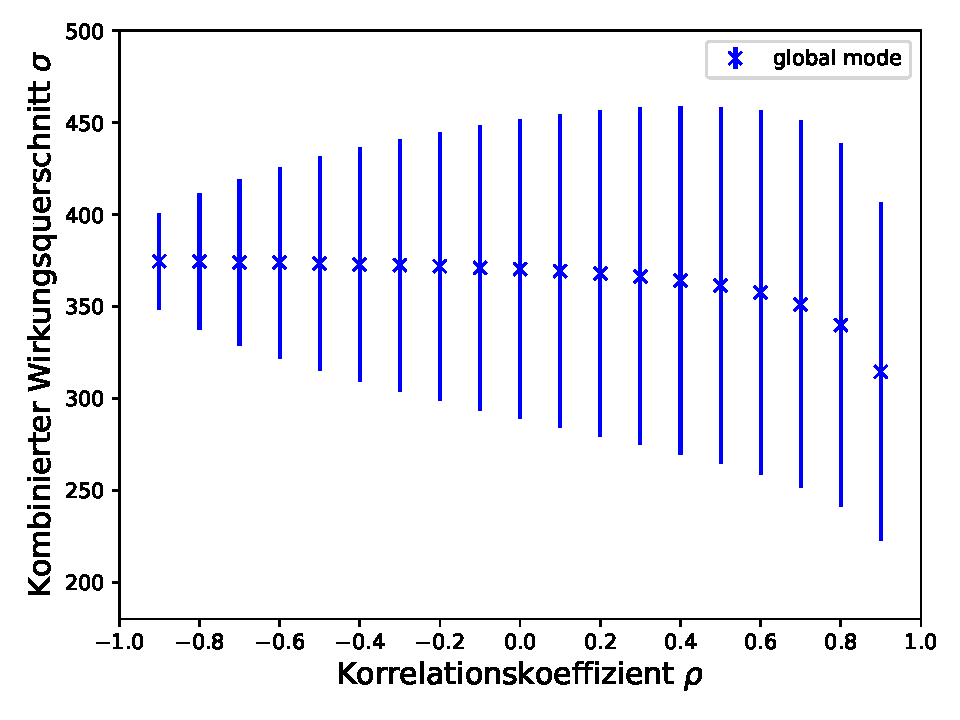
\includegraphics[width=0.7\textwidth]{Plots/corr_CMS.pdf}
  \caption{Untersuchung der Auswirkung verschiedener Korrelationen zwischen $[-0,9~,~0,9]$ zwischen den beiden semileptonischen Produktionswirkungsquerschnittmessungen von CMS.}
  \label{fig:corrcms}
\end{figure}
\begin{figure}
  \centering
  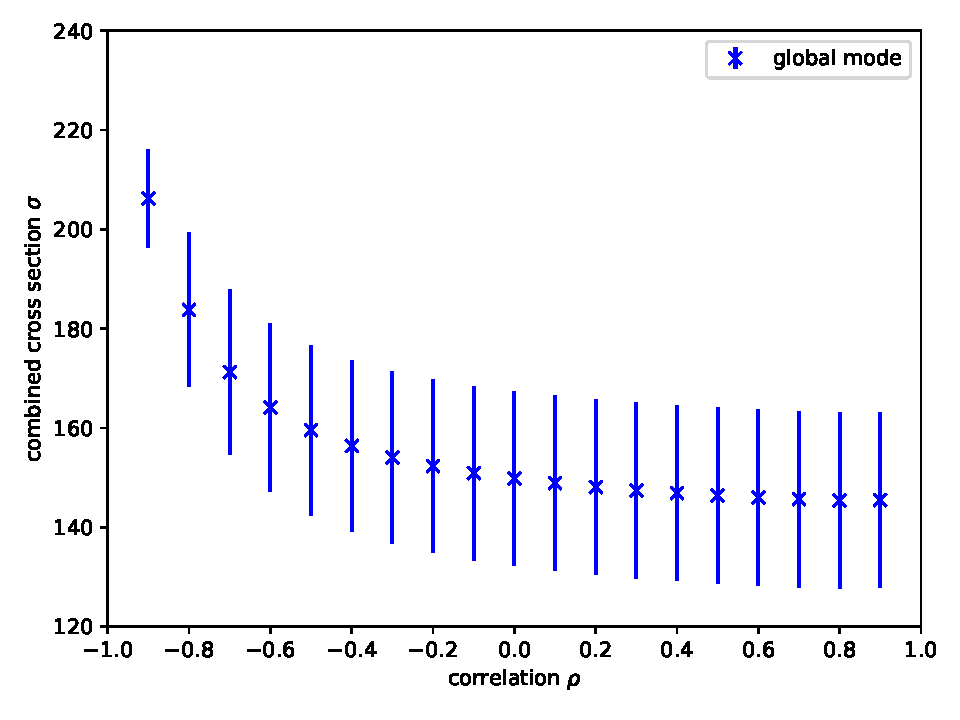
\includegraphics[width=0.7\textwidth]{Plots/fcorr_cms.pdf}
  \caption{Untersuchung der Auswirkung verschiedener Korrelationen zwischen $[-0,9~,~0,9]$ zwischen den beiden semileptonischen Produktionswirkungsquerschnittmessungen von CMS, bei einer Kombination mit der Messung von ATLAS.}
  \label{fig:corrca}
\end{figure}
\begin{figure}
  \centering
  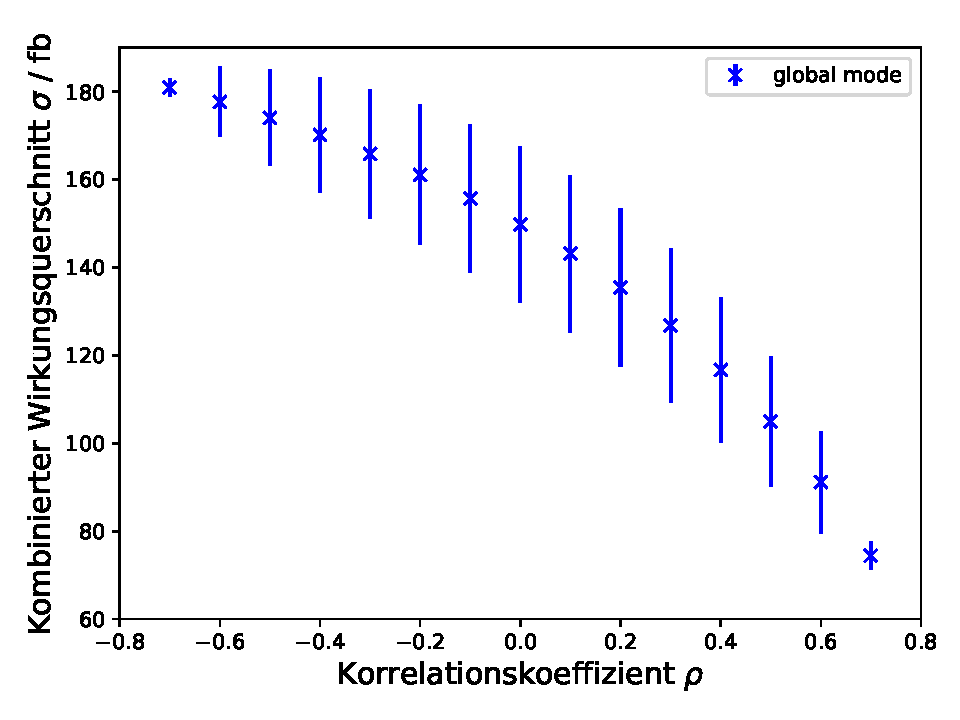
\includegraphics[width=0.7\textwidth]{Plots/corr_CA.pdf}
  \caption{Untersuchung der Auswirkung verschiedener Korrelationen zwischen $[-0,7~,~0,7]$ zwischen den beiden semileptonischen Produktionswirkungsquerschnittmessungen von CMS und der ATLAS Messung.}
  \label{fig:corrCA}
\end{figure}
Zuletzt wird die Korrelation zwischen der ATLAS Messung und den CMS Messungen untersucht. Die dazu verwendete Korrelationsmatrix hat die Form:
\begin{align}
  \text{Corr}_{\sigma,\text{CMS}}\,=\begin{pmatrix}
  1 & \rho_{e, \mu} & \rho_{e, \mu}\\
  \rho_{e, \mu} & 1 &0\\
  \rho_{e, \mu} & 0 & 1
  \end{pmatrix}
  \label{eqn:matrix2}
\end{align}
und die Korrelation wird entsprechend in $0,1$ Schritten im Bereich $[-0,7~,~0,7]$ variiert. In Abbildung~\ref{fig:corrCA} sind die sich ergebenden Ergebnisse dargestellt. Es fällt deutlich auf, dass sich kein Verlauf einstellt, der sich einem gewissen Bereich annähert. Dies deutet darauf hin, dass die Messungen des $t\bar{t}\gamma$ Produktionswirkungsquerschnitts korreliert sind.

\section{Interpretation der Ergebnisse der Kombination}
Zusammenfassend lässt sich feststellen, dass eine unkorrelierte Kombination der drei Messungen des Produktionswirkungsquerschnitts~$t\bar{t}\gamma$ nicht sinnvoll ist.
Dies liegt zum Einen an der Erweiterung des Phasenraums der CMS Messungen und der Extrapolation der Unsicherheiten. Es ist zu vermuten, dass diese im gemessenen Phasenraum von ATLAS nicht gültig sind. Mögliche Lösungen wären zum Einen genauere Rechnungen, um den Faktor $f$ zwischen den Phasenräumen nicht über eine Näherung zwischen LO- und NLO-Rechnungen bestimmen zu müssen. Zum Anderen wäre es möglich die ATLAS Messung des Produktionswirkungsquerschnitts in den CMS Phasenraum zu transformieren. In diesem Fall werden die Unsicherheiten durch die Extrapolation nicht vergrößert, sodass der EFTfitter alle drei Messungen stärker gewichtet.
Zum Anderen zeigen die Ergebnisse aus der Korrelationsstudie, dass die Annahme, dass die Messungen nicht korreliert sind, nur für die beiden CMS Messungen gerechtfertigt ist. Für die Korrelation zwischen der ATLAS und den CMS Messungen bedarf es jedoch noch weiterer Studien.
Da unter den in dieser Arbeit getätigten Annahmen die Kombination der Messungen nahe an dem ATLAS Wert liegt und verschiedene Faktoren dafür sprechen, dass die beiden Messungen hinsichtlich ihrer Unsicherheiten und Korrelationen erst weiter untersucht werden müssen, wird für die weitere Arbeit nur die ATLAS Messung verwendet.
%
%
\chapter{EFT-Modell mit MG5}
In diesem Kapitel erfolgt eine Variation der Wilson-Koeffizienten mit Hilfe eines EFT Modells für MG. Dies ermöglicht die Berechnung eines Modells der Wirkungsquerschnitte für den EFTfitter mit dessen Hilfe später die Wilson-Koeffizienten bestimmt werden können.

\section{Zusammensetzung des Wirkungsquerschnitts}
Der Fit des EFTfitters basiert auf einem funktionellen Zusammenhang zwischen den Observablen, in diesem Fall den Wirkungsquerschnitten, und den Operatoren höherer Ordnung. Diese Abhängigkeit wird durch das implementierte Modell und dem entsprechend mit der Likelihood ausgedrückt.\\
Für die Berechnung des Wirkungsquerschnitts werden alle zugehörigen Feynman-Graphen, sowohl die des SM, als auch die der EFT-Operatoren, betrachtet. Daher ergibt sich der Wirkungsquerschnitt zu:
\begin{align}
  \sigma = \sigma_{SM} + \frac{1}{\Lambda^2} \sum_{i} C_i \sigma_i^\text{interf.} + \frac{1}{\Lambda^4} \sum_{i \leq j} C_i C_j \sigma_{ij}^\text{BSM} + \mathcal{O} \left(\frac{1}{\Lambda^6}\right).
\end{align}
Die einzelnen Wirkungsquerschnitte $\sigma_i$ besitzen eine quadratische Abhängigkeit von den Wilson-Koeffizienten $C_i$ und die BSM-Beiträge in führender Ordnung ergeben sich durch die Interferenz zwischen dem SM und der BSM-Physik. Dies liegt unter Anderem daran, dass die Beiträge durch die Interferenz zwischen den BSM-Physik-Beiträgen untereinander mit $\frac{1}{\Lambda^4}$ unterdrückt sind. Um trotzdem ein möglichst genaues Modell für die Abhängigkeit der Wirkungsquerschnitte von den Wilson-Koeffizienten zu erhalten, müssen auch diese Beiträge betrachtet werden. Dies wurde bereits in dem Papier\cite{Wilson-Beiträge} untersucht. Zur Bestimmung des Modells ist es zudem notwendig die Wirkungsquerschnitte für verschiedene Konfigurationen der Wilson-Koeffizienten zu bestimmen.

\section{Variation der Wilson-Koeffizienten mit MadGraph5}
Eine Möglichkeit die Wilson-Koeffizienten zu variieren ist mit Hilfe eines MG Modells, dass Operatoren der Massendimension sechs enthält und damit eine Berechnung der Wirkungsquerschnitte unter dem Einfluss dieser ermöglicht. Dazu wird in MadGraph5 das TEFT\_EF UFO Modell\cite{EFTModell} eingebunden. Dies erlaubt NLO Rechnung in der QCD und enthält alle für die Top-Quark-Physik relevanten Operatoren der Dimension sechs.\\
Die Berechnung erfolgt mit dem genannten Modell in NLO in QCD unter der Verwendung des $\text{CTEQ}6\text{L}1$ PDF Sets. Zudem wird die Energieskala auf $\SI{1}{\tera\electronvolt}$ festgelegt. Unter diesen Vorraussetzungen wird der Prozess $pp~\rightarrow~t\bar{t}~\gamma$ mit den von ATLAS genutzten Schnitten implementiert.\\
Da die Berechnung statistische Unsicherheiten enthält, bietet es sich an anstatt nur genügend viele Berechnungen der Monte Carlo Wirkungsquerschnitte $\sigma_{MC}$ für ein bestimmtes Gleichungssystem zur Bestimmung der Wirkungsquerschnitte $\sigma_i$ durchzuführen sondern mehr. Zudem werden genauere Ergebnisse erhalten, wenn sowohl Berechnungen bei denen nur ein Wilson-Koeffizient angeschaltet ist, als auch welche beidenen mehrere oder sogar alle betrachtet werden, getätigt werden.\\
Die berechneten Monte Carlo Wirkungsquerschnitte:
\begin{align}
  \sigma_{MC}({C_i}) = \sigma_{SM} + \sum_{i} C_i \frac{\sigma_i}{\Lambda^2} + \sum_{i \leq j} C_i C_j \frac{\sigma_{ij}}{\Lambda^4} + \mathcal{O}(\frac{1}{\Lambda^6})
\end{align}
bilden die Stützstellen zur späteren Bestimmung der gesuchten Wirkungsquerschnitte. Mit Hilfe des Vakuumerwartungswert des Higgs $\SI{246}{\giga\electronvolt}$ und der Wahl $\Lambda = \SI{1}{\tera\electronvolt}$ lassen sich die $\sigma_{MC}$ in natürliche Einheiten umrechnen. Unter Vernachlässigung de Terme der Ordnung $\mathcal{O}(\frac{1}{\Lambda^6})$ ergeben sie sich zu:
\begin{align}
  \sigma_{MC}({\tilde{C_i}}) \approx \bar{\sigma}_{SM} + \sum_{i} \tilde{C_i} \bar{\sigma_i} + \sum_{i \leq j} \tilde{C_i} \tilde{C_j} \bar{\sigma}_{ij}.
\end{align}
Hierbei sind die $\tilde{C}_i = \frac{v^2}{\Lambda^2} C_i$.
Bei der Berechnung des $t\bar{t}\gamma$ Produktionswirkungsquerschnitts können, wie in Kapitel~\ref{top} bereits erwähnt, die Operatoren $O_{tG}$, $O_{tW}$ und $O_{tB}$ beitragen. Damit ergibt sich die Interpolationsfunktion zu:
\begin{align}
  \sigma_{t\bar{t}\gamma, MC}({\tilde{C}_{tG}, \tilde{C}_{tW}, \tilde{C}_{tB}}) = \bar{\sigma}_{SM} + \tilde{C}_{tG}\bar{\sigma}_{tG} + \tilde{C}_{tW}\bar{\sigma}_{tW} + \tilde{C}_{tB}\bar{\sigma}_{tB}\\
  + \tilde{C}_{tG}^2\bar{\sigma}_{tGtG} + \tilde{C}_{tW}^2\bar{\sigma}_{tWtW} + \tilde{C}_{tB}^2\bar{\sigma}_{tBtB}\\
  + \tilde{C}_{tG} \tilde{C}_{tW}\bar{\sigma}_{tGtW} + \tilde{C}_{tG} \tilde{C}_{tB}\bar{\sigma}_{tGtB} + \tilde{C}_{tW} \tilde{C}_{tB}\bar{\sigma}_{tWtB}
\end{align}
und es müssen insgesamt zehn Parameter $\bar{\sigma_i}$ und $\bar{\sigma}_{ij}$ bestimmt werden. Dazu werden die Wilson-Koeffizienten $C_{tG}$, $C_{tW}$ und $C_tB$ im Bereich $[-30~,~30]$ variiert. Um erneut nur die semileptonischen Endzustände zu betrachten, müssen auch in diesem Fall die $\sigma_{t\bar{t}\gamma, MC}$ mit dem $\mathrm{BR} = \SI{30}{\percent}$ multipliziert werden. Aus diesen Berechnungen lassen sich dann mit der Methode der kleinsten Quadrate die gesuchten Parameter bestimmen, aus denen sich schließlich das Modell für den EFTfitter ergibt.

\section{Plots mit Schnitten}
Die Schnitte mit der sich ergebenen Hyperebene sind parabelförmig, wenn nur ein Wilson-Koeffizient variiert wird. Dies ist zu erwarten, da die Zusammensetzung der Monte Carlo Wirkungsquerschnitt auch aus quadratischen Anteilen besteht. Die direkt an der Photonabstrahlung beteiligten Wilson-Koeffizienten $C_{tW}$ und $C_{tB}$ folgen ziemlich genau diesem parabelförmigen Verlauf. Dies ist in Abbildung~\ref{fig:WtW} und~\ref{fig:WtB} veranschaulicht. Lediglich die berechneten Wirkungsquerschnitte für den Wilson-Koeffizienten $C_{tG}$ weisen stärke Abweichungen auf, dies ist in Abbildung~\ref{fig:WtG} dargestellt.\\
Die Ursache hierfür könnte bei (...)liegen.
\begin{figure}
  \begin{subfigure}[c]{0.5\textwidth}
    \centering
    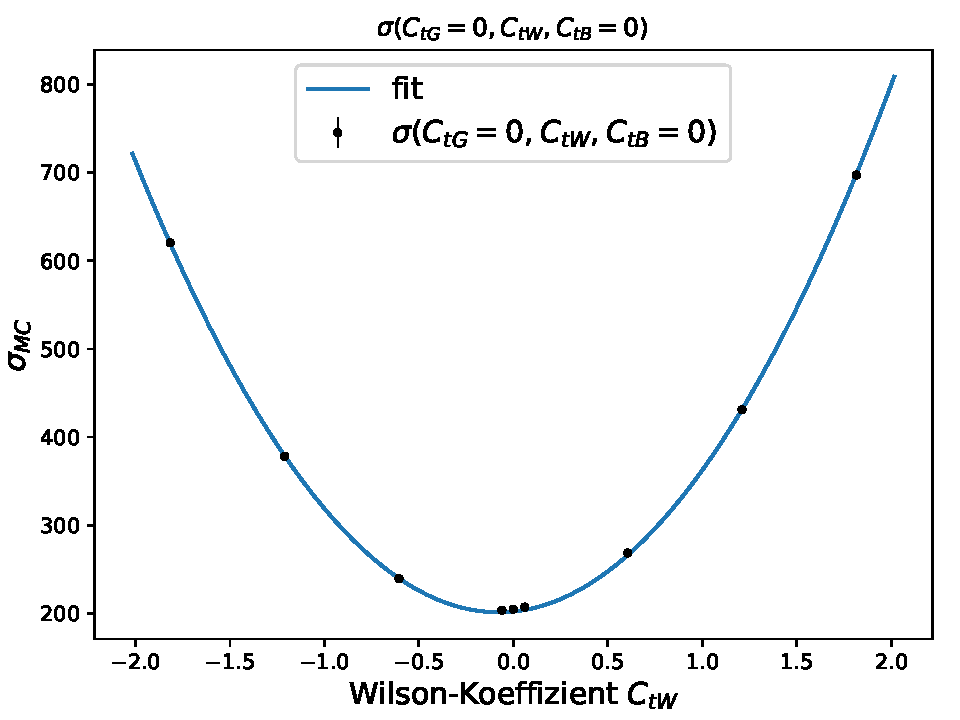
\includegraphics[width=\textwidth]{Plots/combi_plot_tW.pdf}
    \subcaption{Verlauf für $C_tW$ mit $C_{tB}=C_{tG}=0$.}
    \label{fig:WtW}
  \end{subfigure}
  \begin{subfigure}[c]{0.5\textwidth}
    \centering
    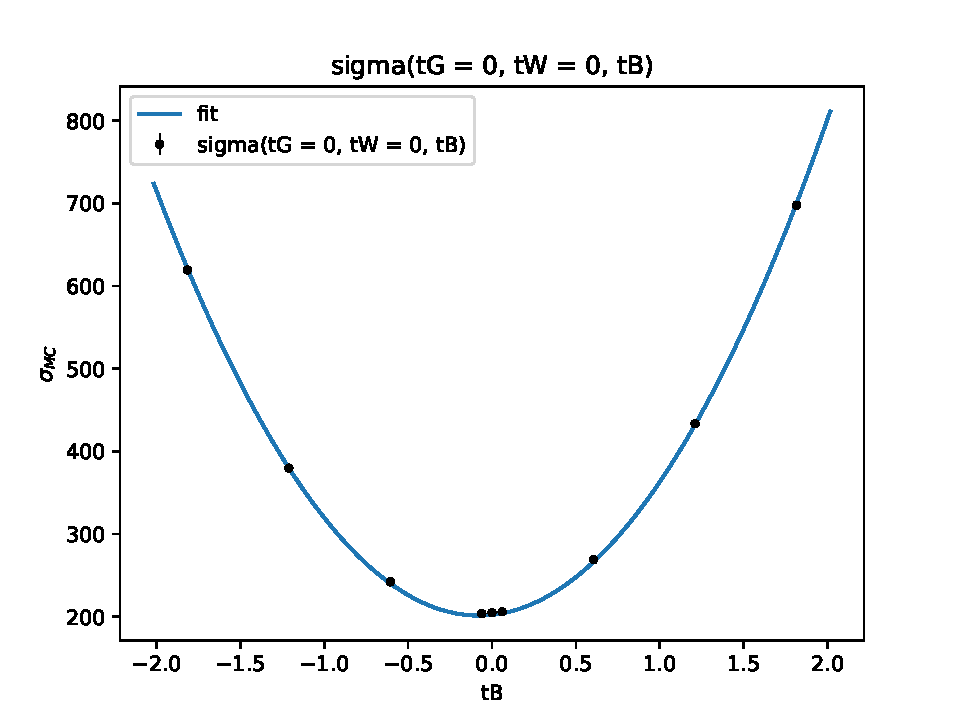
\includegraphics[width=\textwidth]{Plots/combi_plot_tB.pdf}
    \subcaption{Verlauf für $C_tB$ mit $C_{tW}=C_{tG}=0$.}
    \label{fig:WtB}
  \end{subfigure}
  \caption{Graphische Darstellung des parabelförmigen Verlaufs der Wirkungsquerschnitte für die Betrachtung einzelner Wilson-Koeffizienten.}
\end{figure}
\begin{figure}
  \centering
  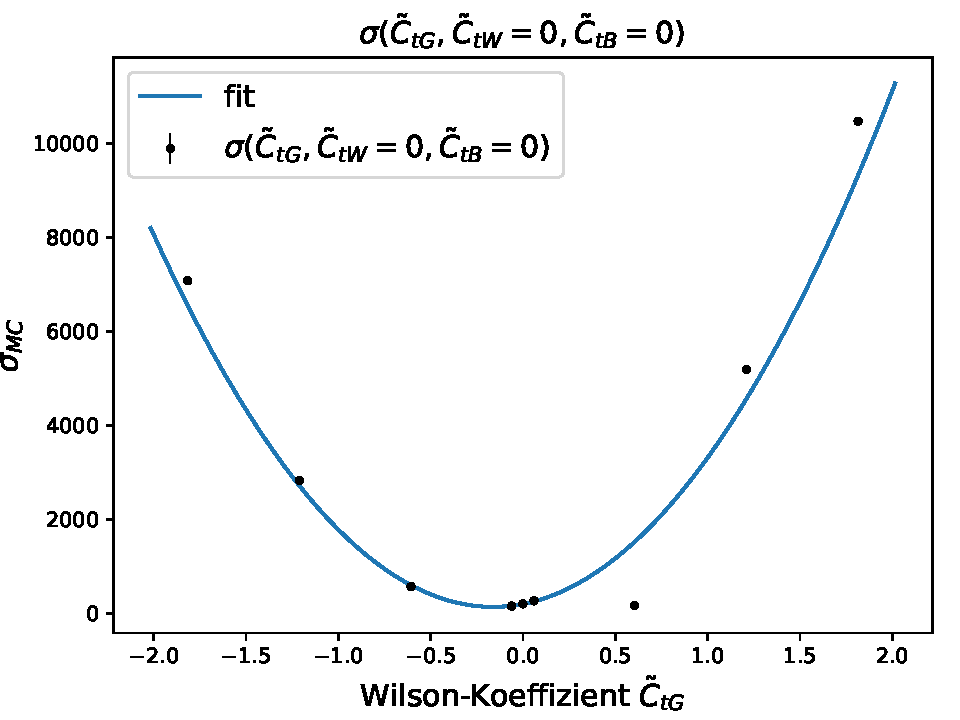
\includegraphics[width=0.5\textwidth]{Plots/combi_plot_tG.pdf}
  \caption{Graphische Darstellung des parabelförmigen Verlaufs der Wirkungsquerschnitte für den Wilson-Koeffizienten $C_{tG}$, wenn $C_{tW}=C_{tB}=0$ ist.}
  \label{fig:WtG}
\end{figure}

\section{MadGraph Modell für den EFTfitters}
\begin{align*}
  s_{SM}   &= 202.193110217 \pm 0.0293749106165\\
  s_tW   &= 21.6894366072 \pm 0.279039825848\\
  s_tB   &= 761.416032917 \pm 8.2990258513\\
  s_tG   &= 21.6811677276 \pm 0.337443892498\\
  s_tWtW &= 11.7700260688 \pm 0.000323156142251\\
  s_tBtB &= 48.4373822429 \pm 0.00172124829635\\
  s_tGtG &= 11.794900333 \pm 0.000390544938718\\
  s_tBtW &= 279.22019759 \pm 1.61033246225\\
  s_tWtG &= 6863.75881087 \pm -1.44115188502e+17\\
  s_tBtG &= -6483.30787401 \pm -1.4411518765e+17
\end{align*}
\textit{Die Frage ist hier halt ob diese angegebenen Fehler überhaupt aussagekräftig sind. Das ist ja eine statistische Abschätzung, die auch gewissen Annahmen beinhaltet.Bei einem so hochdimensionalem Fit ist das natürlich auch sehr anfällig bei Abweichungen.. und die sind besonders im Fall von $C_tG$ ja offensichtlich noch vorhanden.}
%
%
\chapter{EFT-Interpretation des \texorpdfstring {$t\bar{t}\gamma$}{math} Produktionswirkungsquerschnitts mit dem EFTfitter}

\section{Ergebnis für die Wilson-Koeffizienten}

\begin{figure}
    \centering
    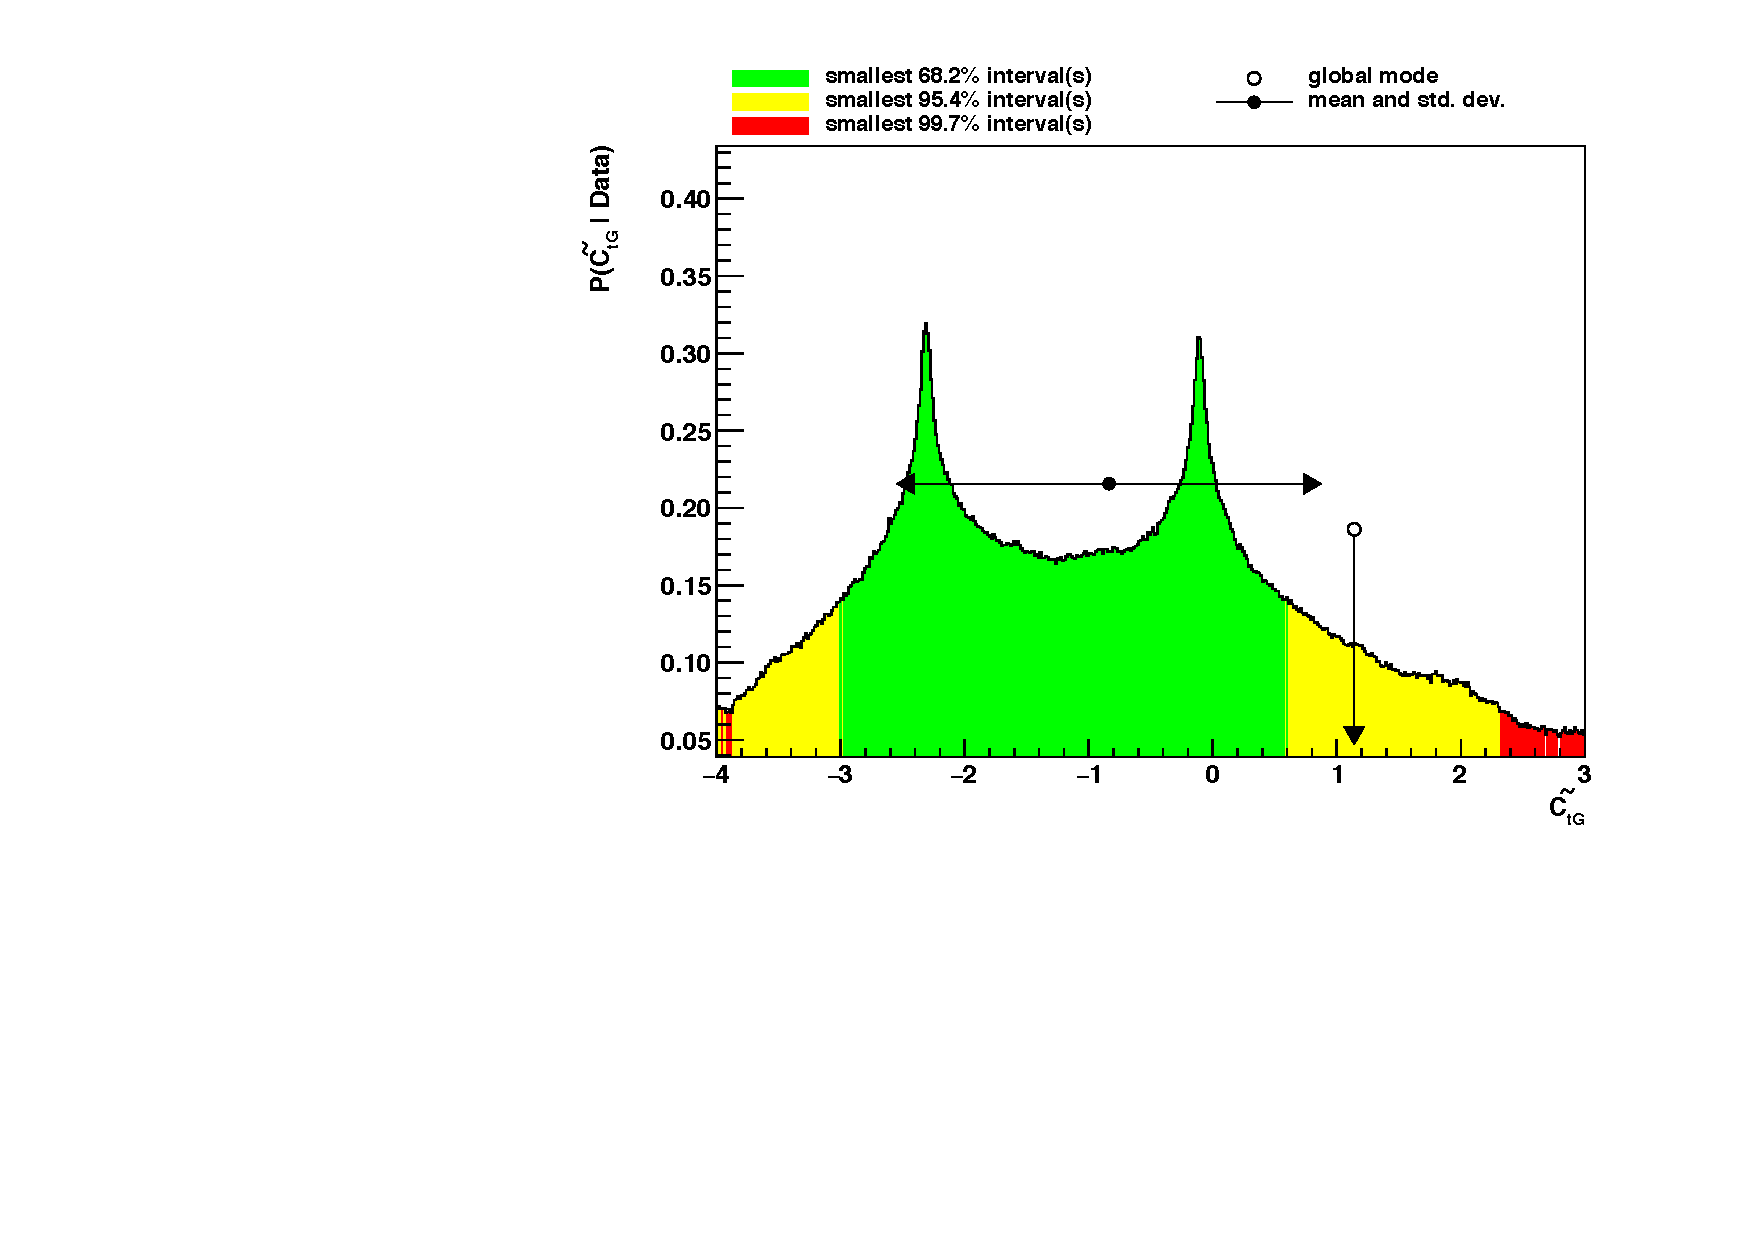
\includegraphics[width=0.8\textwidth]{Plots/result_CtG.pdf}
\end{figure}
\begin{figure}
    \centering
    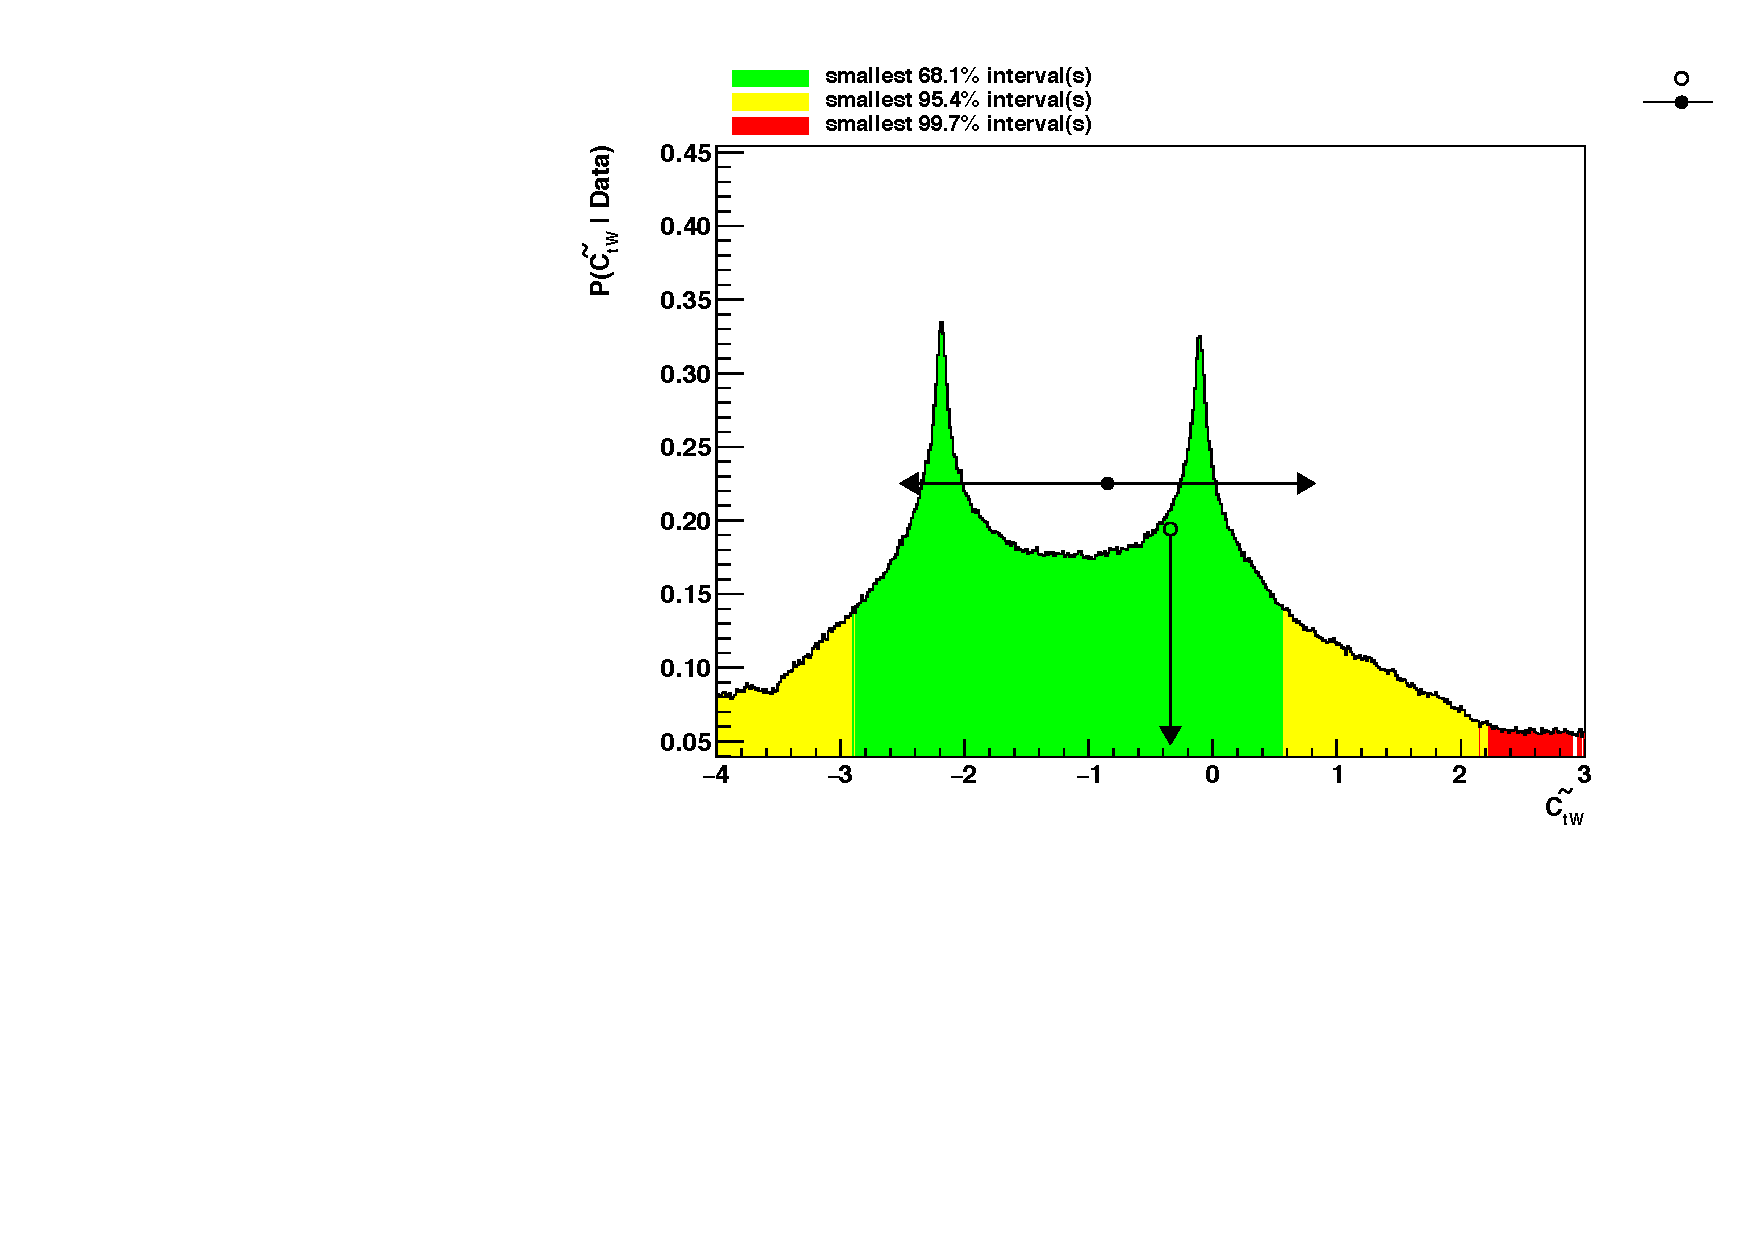
\includegraphics[width=0.8\textwidth]{Plots/result_CtW.pdf}
\end{figure}
\begin{figure}
    \centering
    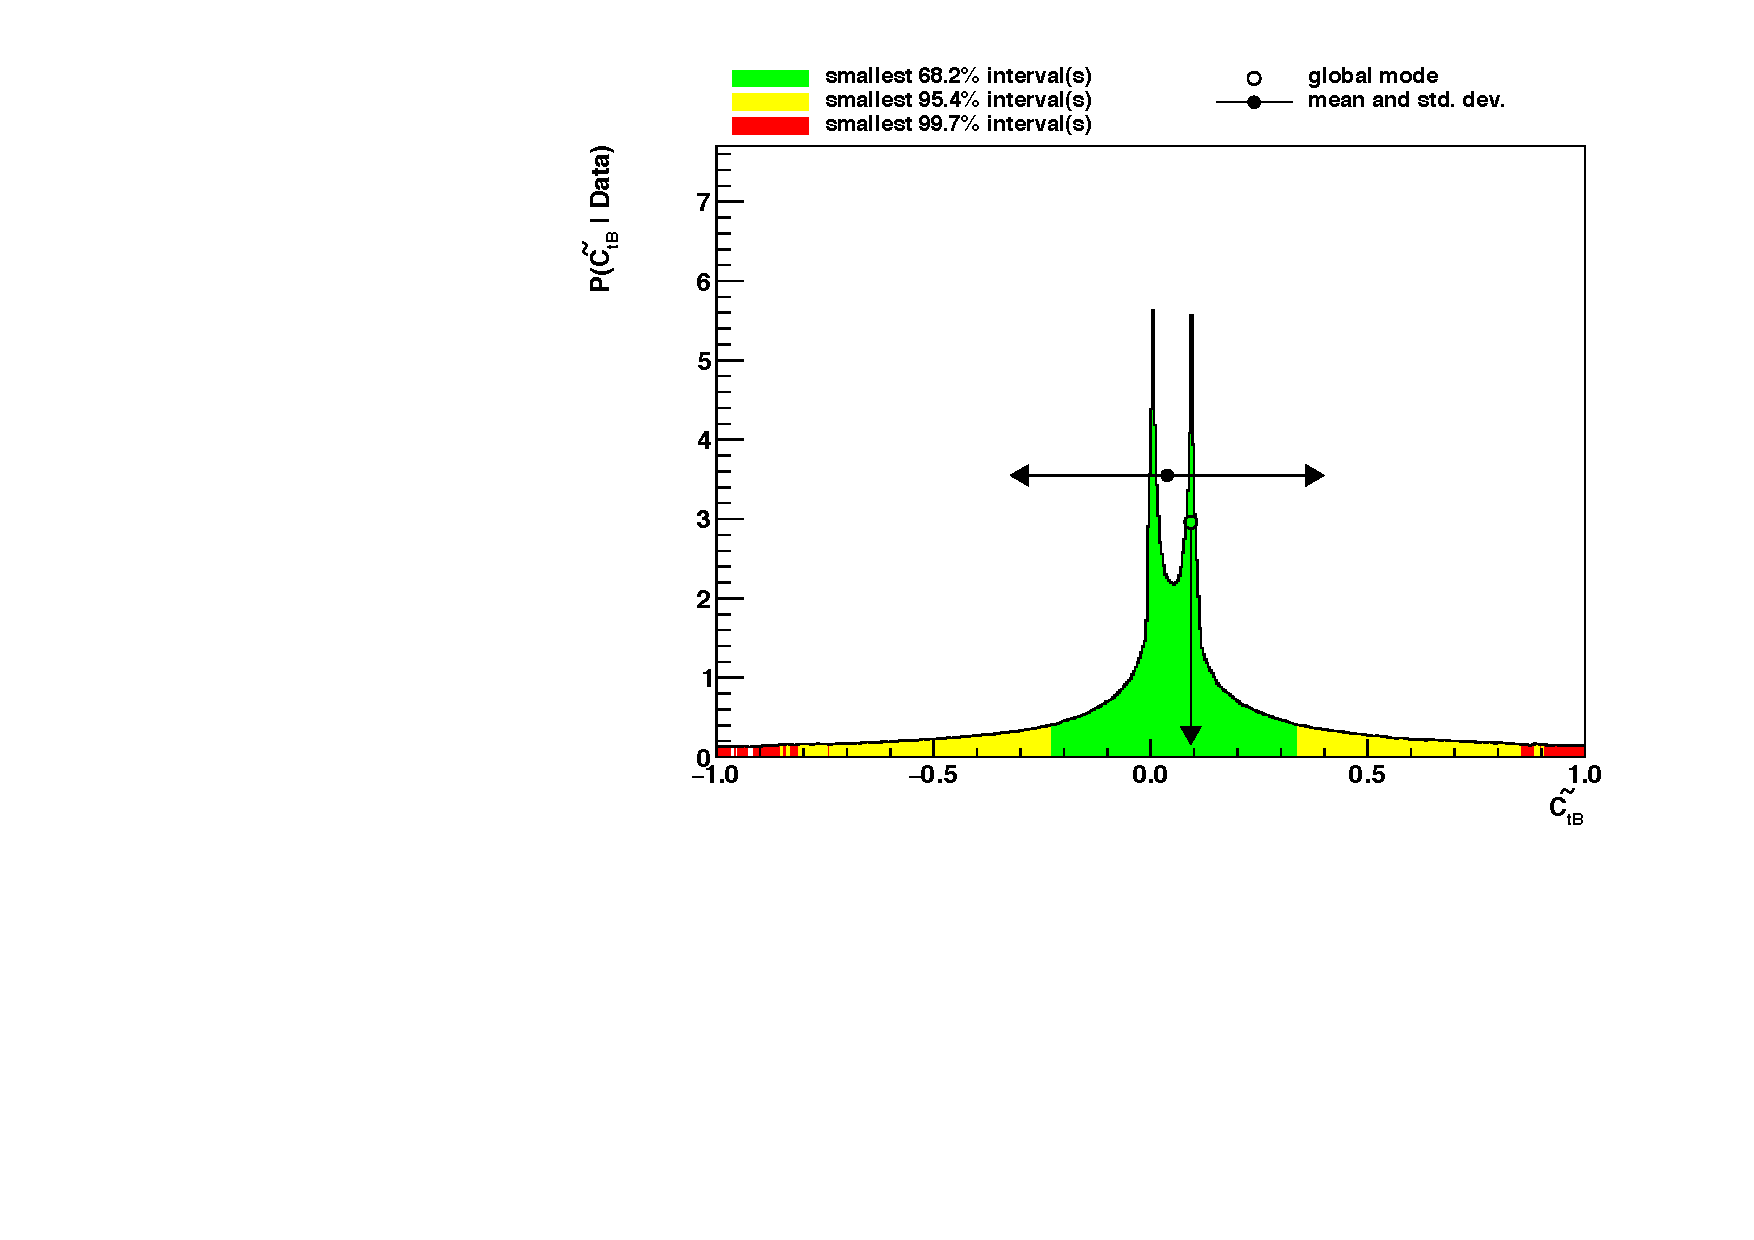
\includegraphics[width=0.8\textwidth]{Plots/result_CtB.pdf}
\end{figure}

\chapter{EFT-Modell mit MadGraph5}
In diesem Kapitel erfolgt eine Variation der Wilson-Koeffizienten mit Hilfe  von MadGraph5 unter der Verwendung eines EFT-Modells. Dies ermöglicht die Berechnung eines approximierten Modells der Wirkungsquerschnitte für den EFT\textit{fitter} mit dessen Hilfe die Wilson-Koeffizienten bestimmt werden können. Dieses approximierte Modell wird benötigt, um die Laufzeiten des EFT\textit{fitter} zu verringern.

\section{Wirkungsquerschnitt}
Der Fit des EFT\textit{fitter}s basiert auf einem funktionellen Zusammenhang zwischen den Observablen, in diesem Fall den Wirkungsquerschnitten, und den Operatoren höherer Ordnung. Diese Abhängigkeit wird durch das implementierte Modell in einer Likelihood ausgedrückt. Diese Likelihood wird mit einer Approximation durch MG bestimmt, da die Laufzeit des EFT\textit{fitter}s dadurch deutlich geringer wird.\\
Für die Berechnung des Wirkungsquerschnitts werden die zugehörigen Feynman-Graphen, sowohl die des SM, als auch die der EFT-Operatoren, betrachtet. Damit ergibt sich die Approximation des Wirkungsquerschnittes zu:
\begin{align}
  \sigma = \sigma_{SM} + \frac{1}{\Lambda^2} \sum_{i} C_i \sigma_i^\text{interf.} + \frac{1}{\Lambda^4} \sum_{i \leq j} C_i C_j \sigma_{ij}^\text{BSM} + \mathcal{O} \left(\frac{1}{\Lambda^6}\right).
\end{align}
Die einzelnen Wirkungsquerschnitte $\sigma$ besitzen eine quadratische Abhängigkeit von den Wilson-Koeffizienten $C_i$ und die BSM-Beiträge in führender Ordnung ergeben sich durch die Interferenz zwischen dem SM und der BSM-Physik. Dies liegt unter anderem daran, dass die Beiträge durch die BSM-Physik-Beiträge alleine mit $\frac{1}{\Lambda^4}$ unterdrückt sind. Untersuchungen~\cite{Fichet:2016iuo} haben ergeben, dass diese Beiträge trotzdem betrachtet werden sollten, um ein Modell für die Abhängigkeit der Wirkungsquerschnitte von den Wilson-Koeffizienten zu erhalten, da sie zur Genauigkeit des Modells beitragen.

\section{Variation der Wilson-Koeffizienten in MadGraph5}%
%
Zur Bestimmung dieses Modells ist es notwendig, die Wirkungsquerschnitte für verschiedene Konfigurationen der Wilson-Koeffizienten zu bestimmen, um sowohl den Einfluss einzelner als auch mehrerer Operatoren untersuchen zu können.
Eine Möglichkeit die Wilson-Koeffizienten zu variieren, ist mit Hilfe eines  EFT-Modells für MG, das Operatoren der Massendimension sechs enthält und damit eine Berechnung der Wirkungsquerschnitte unter dem Einfluss dieser Operatoren ermöglicht. Dazu wird in MG das TEFT\_EF UFO Modell~\mcite{Bylund:2016phk, Franzosi:2015osa, Zhang:2016omx, Degrande:2011ua} eingebunden.
Dies enthält einige der für die Top-Quark-Physik relevanten Operatoren der Dimension sechs und insbesondere die, die an dem Prozess $pp~\rightarrow~t\bar{t}~\gamma$ beteiligt sind.
Die Berechnung erfolgt mit dem genannten Modell in NLO in QCD unter der Verwendung des $\text{CTEQ}6\text{L}1$ PDF-Satzes.
Zudem wird die BSM-Energieskala auf $\Lambda = \SI{1}{\tera\electronvolt}$ festgelegt.
Unter diesen Vorraussetzungen wird der Prozess $pp~\rightarrow~t\bar{t}~\gamma$ mit den von ATLAS genutzten Schnitten für den gemessenen Phasenraum implementiert.\\
Die berechneten Monte-Carlo-Wirkungsquerschnitte:
\begin{align}
  \sigma_{MC}({C_i}) = \sigma_{SM} + \sum_{i} C_i \frac{\sigma_i}{\Lambda^2} + \sum_{i \leq j} C_i C_j \frac{\sigma_{ij}}{\Lambda^4} + \mathcal{O}\left(\frac{1}{\Lambda^6}\right)
\end{align}
bilden die Stützstellen zur späteren Bestimmung der gesuchten Parameter $\sigma_i$ und $\sigma_{ij}$.
Mit Hilfe des Vakuumerwartungswerts des Higgs-Feldes $v = \SI{246}{\giga\electronvolt}$ und der Wahl $\Lambda = \SI{1}{\tera\electronvolt}$ lassen sich die $\sigma_{MC}$ in die Größenordnung einer Kopplungsstärke umrechnen.
Unter Vernachlässigung von Termen der Ordnung $\mathcal{O}(\frac{1}{\Lambda^6})$, ergeben sie sich zu:
\begin{align}
  \sigma_{MC}({\tilde{C_i}}) \approx \sigma_{SM} + \sum_{i} \tilde{C_i} \bar{\sigma_i} + \sum_{i \leq j} \tilde{C_i} \tilde{C_j} \bar{\sigma}_{ij}.
\end{align}
Hierbei sind die $\tilde{C}_i = \frac{v^2}{\Lambda^2} C_i$, $\bar{\sigma}_i = \frac{\sigma_i}{v^2}$ und $\bar{\sigma}_{ij} = \frac{\sigma_{ij}}{v^4}$ die zugehörgen Parameter.
Bei der Berechnung des $t\bar{t}\gamma$ Produktionswirkungsquerschnitts können, wie in Kapitel~\ref{top} bereits erwähnt, die Operatoren $O_{tG}$, $O_{tW}$ und $O_{tB}$ beitragen. Damit ergibt sich die Interpolationsfunktion zu:
\begin{align}
  \sigma_{t\bar{t}\gamma, MC}({\tilde{C}_{tG}, \tilde{C}_{tW}, \tilde{C}_{tB}}) = \sigma_{SM} + \tilde{C}_{tG}\bar{\sigma}_{tG} + \tilde{C}_{tW}\bar{\sigma}_{tW} + \tilde{C}_{tB}\bar{\sigma}_{tB}\\ \nonumber
  + \tilde{C}_{tG}^2\bar{\sigma}_{tGtG} + \tilde{C}_{tW}^2\bar{\sigma}_{tWtW} + \tilde{C}_{tB}^2\bar{\sigma}_{tBtB}\\
  + \tilde{C}_{tG} \tilde{C}_{tW}\bar{\sigma}_{tGtW} + \tilde{C}_{tG} \tilde{C}_{tB}\bar{\sigma}_{tGtB} + \tilde{C}_{tW} \tilde{C}_{tB}\bar{\sigma}_{tWtB} \nonumber
\end{align}
und es müssen insgesamt zehn Parameter $\bar{\sigma_i}$ und $\bar{\sigma}_{ij}$ bestimmt werden. Dazu werden die Wilson-Koeffizienten $C_{tG}$, $C_{tW}$ und $C_{tB}$ im Bereich $[-30~,~30]$ variiert. Auf Grund der statistischen Unsicherheiten werden insgesamt $50$ verschiedene Variationen durchgeführt, bei denen ein, zwei oder alle der Wilson-Koeffizienten ungleich Null sind.
Um erneut nur die Lepton+Jets-Endzustände zu betrachten, müssen auch in diesem Fall die $\sigma_{t\bar{t}\gamma, MC}$ mit dem Verzweigungsverhältnis für Lepton+Jets-Ereignisse $\mathrm{BR} \approx \SI{30}{\percent}$ multipliziert werden.
Aus diesen Berechnungen lassen sich dann mit der Methode der kleinsten Quadrate die gesuchten Parameter bestimmen, aus denen sich schließlich das Modell für den EFT\textit{fitter} ergibt.


\section{Bestimmung des Modells für den EFT\textit{fitter}}
\label{Modell}
Durch die Bestimmung der gesuchten Parameter mit der Methode der kleinsten Quadrate werden die folgenden Wirkungsquerschnitte bestimmt:
\begin{table}[H]
    \centering
   \begin{tabular}{ll}
     $\sigma_{SM}   = \SI{202.19}{\femto\barn\per\giga\electronvolt\squared} $  & $\bar{\sigma}_{tW}   = \SI{21.7}{\femto\barn\per\giga\electronvolt\squared}$\\
     $\bar{\sigma}_{tB}   = \SI{21.7}{\femto\barn\per\giga\electronvolt\squared}$    & $\bar{\sigma}_{tG}   = \SI{761.4}{\femto\barn\per\giga\electronvolt\squared}$\\
     $\bar{\sigma}_{tWtW} = \SI{11.7}{\femto\barn\per\giga\electronvolt\tothe{4}}$    & $\bar{\sigma}_{tBtB} = \SI{11.8}{\femto\barn\per\giga\electronvolt\tothe{4}}$\\
     $\bar{\sigma}_{tGtG} = \SI{48.4}{\femto\barn\per\giga\electronvolt\tothe{4}}$    & $\bar{\sigma}_{tGtW} = \SI{6863.8}{\femto\barn\per\giga\electronvolt\tothe{4}}$\\
     $\bar{\sigma}_{tGtB} = \SI{-6483.3}{\femto\barn\per\giga\electronvolt\tothe{4}}$ & $\bar{\sigma}_{tWtB} = \SI{279.2}{\femto\barn\per\giga\electronvolt\tothe{4}}$
   \end{tabular}
\end{table}
Die Unsicherheiten aus dem Fit mit der Methode der kleinsten Quadrate werden hier vernachlässigt, da diese nicht im Modell des EFT\textit{fitter}s implementiert werden können. Die gültigen Stellen orientieren sich an der Fehlern, der berechneten Stützstellen.\\
In den Abbildungen~\ref{fig:tp} und~\ref{fig:WtG} ist erkennbar, dass der Fit die erwartete quadratische Form in den jeweiligen Parametern aufweist. Die für die beiden Wilson-Koeffizienten $\tilde{C}_{tW}$ und $\tilde{C}_{tB}$ berechneten Wirkungsquerschnitte folgen dem erwarteten parabelförmigen Verlauf, wie in Abbildung~\ref{fig:WtW} und~\ref{fig:WtB} veranschaulicht. Die beiden Wilson-Koeffizienten, die zu den beiden an der Photonabstrahlung beteiligten Operatoren gehören, tragen gleich bei. Dies war zuerwarten, da theoretische Berechnungen bewiesen haben, dass die beiden Operatoren $\tilde{O}_{tW}$ und $\tilde{O}_{tB}$ ununterscheidbar sind~\cite{Bylund:2016phk}. Lediglich die berechneten Wirkungsquerschnitte für den Wilson-Koeffizienten $\tilde{C}_{tG}$ weisen teilweise Abweichungen von dem parabelförmigen Verlauf auf, wie in Abbildung~\ref{fig:WtG} erkennbar ist. Zudem fällt auf, dass der Wertebreich der Wirkungsquerschnitte deutlich höher ist, als bei den Wilson-Koeffizienten $\tilde{C}_{tW}$ und $\tilde{C}_{tB}$.\\
Der Fit für den Wilson-Koeffizienten $\tilde{C}_{tG}$ in Abbildung~\ref{fig:WtG} könnte verbessert werden, indem mehr Stützstellen berechnet werden.\\
\begin{figure}
  \begin{subfigure}[c]{0.5\textwidth}
    \centering
    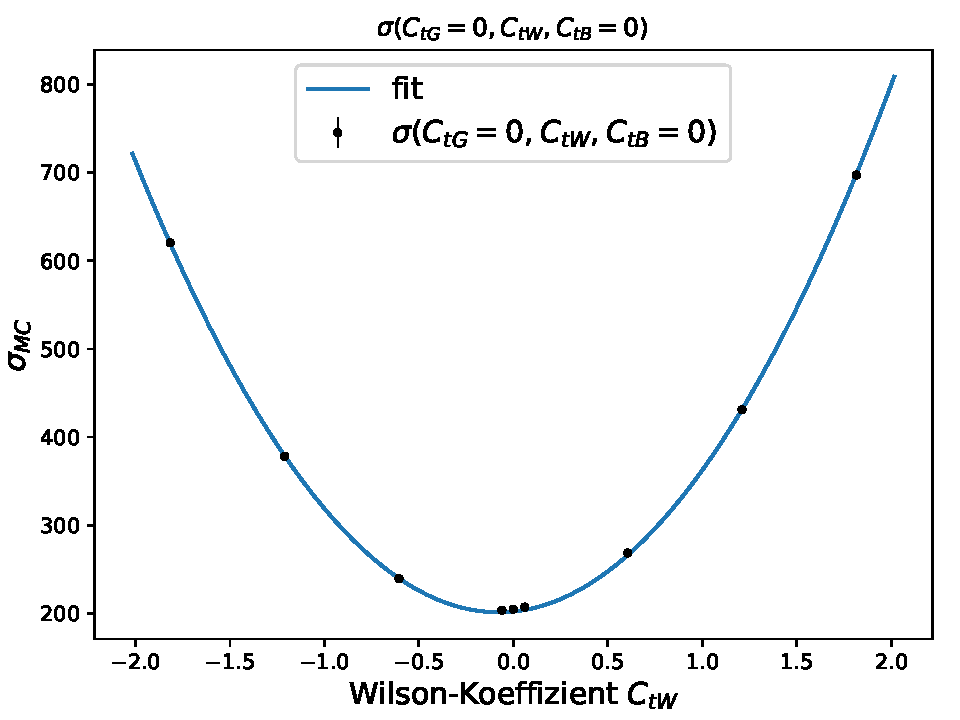
\includegraphics[width=\textwidth]{Plots/combi_plot_tW.pdf}
    \subcaption{Verlauf für $\tilde{C}_{tW}$ mit $\tilde{C}_{tB}=\tilde{C}_{tG}=0$.}
    \label{fig:WtW}
  \end{subfigure}
  \begin{subfigure}[c]{0.5\textwidth}
    \centering
    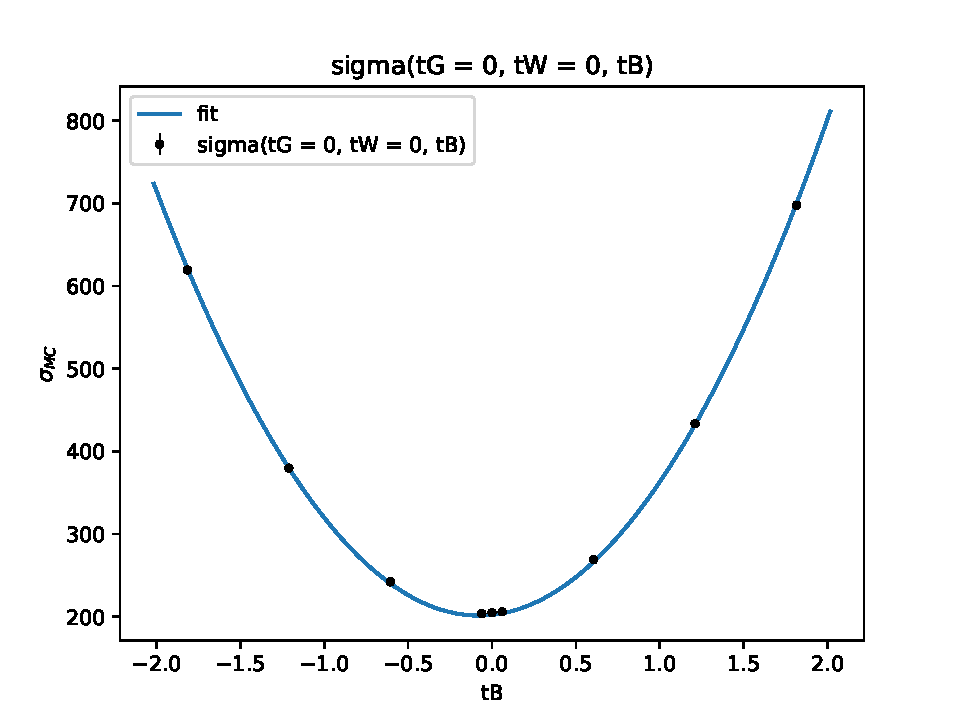
\includegraphics[width=\textwidth]{Plots/combi_plot_tB.pdf}
    \subcaption{Verlauf für $\tilde{C}_{tB}$ mit $\tilde{C}_{tW}=\tilde{C}_{tG}=0$.}
    \label{fig:WtB}
  \end{subfigure}
  \caption{Graphische Darstellung des parabelförmigen Verlaufs der Wirkungsquerschnitte für die Betrachtung einzelner Wilson-Koeffizienten.}
  \label{fig:tp}
\end{figure}
\begin{figure}
  \centering
  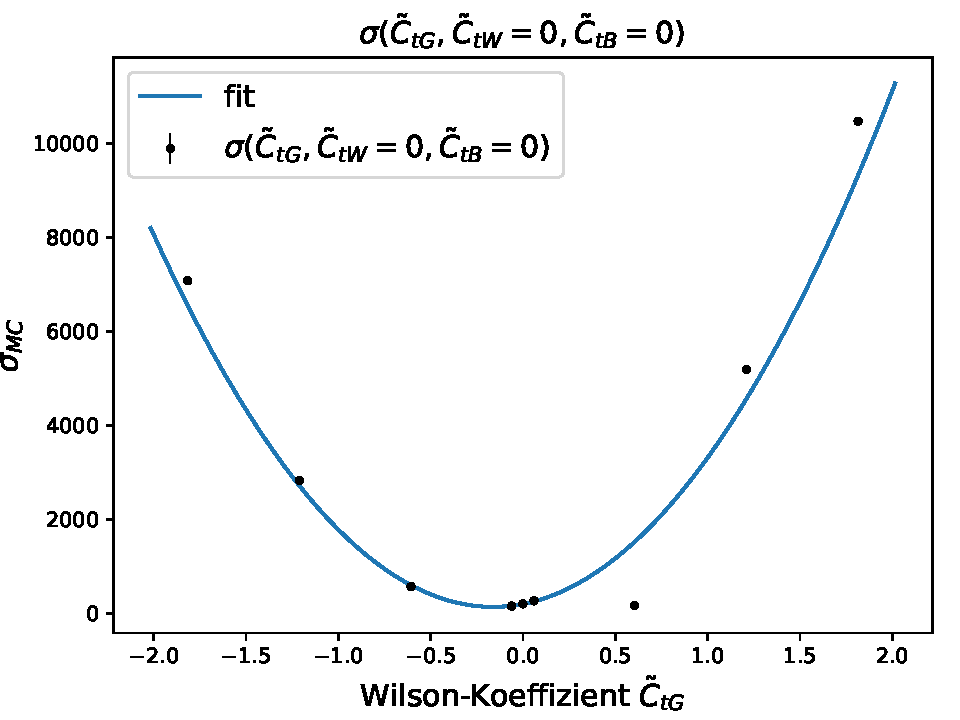
\includegraphics[width=0.6\textwidth]{Plots/combi_plot_tG.pdf}
  \caption{Graphische Darstellung des parabelförmigen Verlaufs der Wirkungsquerschnitte für den Wilson-Koeffizienten $\tilde{C}_{tG}$, wenn $\tilde{C}_{tW}=\tilde{C}_{tB}=0$ gilt.}
  \label{fig:WtG}
\end{figure}
%
%
\chapter{EFT-Interpretation des \texorpdfstring {$t\bar{t}\gamma$}{math}-Produktionswirkungsquerschnitts}
In diesem Kapitel erfolgt die Untersuchung der am $t\bar{t}\gamma$-Produktionswirkungsquerschnitt beteiligten Wilson-Koeffizienten mit dem EFT\textit{fitter}. Dazu wird das mit MadGraph bestimmte Modell aus Kapitel~\ref{Modell} im EFT\textit{fitter} implemeniert und mit Hilfe der ATLAS-Messung die Wilson-Koeffizienten eingeschränkt.

\section{Einschränkung der Wilson-Koeffizienten}
 Der von ATLAS gemessene $t\bar{t}\gamma$-Produktionswirkungsquerschnitt kann mit Hilfe des EFT\textit{fitter} auf mögliche Abweichungen durch die EFT-Operatoren $O_{tG}$, $O_{tW}$ und $O_{tB}$ getestet werden. Dazu wird das in Kapitel~\ref{Modell} berechnete Modell verwendet. Es ermöglicht Einschränkungen für die Wilson-Koeffizienten der EFT-Operatoren zu finden.
In den Abbildungen~\ref{fig:ctw},~\ref{fig:ctb} und~\ref{fig:ctg} sind die marginalisierten, eindimensionalen Posteriorverteilung der Wilson-Koeffizienten, die mit Hilfe des EFT\textit{fitter}s berechnet wurden, dargestellt.
Da der Fit mit einem quadratischen Modell in den Wilson-Koeffizienten durchgeführt wird, stimmt die Messung an zwei Stellen mit der Vorhersage überein, sodass sich zwei Peaks ergeben.
Da für jeden Wilson-Koeffizienten eines der Maxima in der Nähe von Null liegt und das kleinste $\SI{68.1}{\percent}$-Intervall diesen Wert umfasst, kann die SM Vorhersage, dass die Wilson-Koeffizienten Null sind, nicht verworfen werden.
Das $\SI{68.1}{\percent}$-Intervall ist für alle Wilson-Koeffizient in Abbildung~\ref{fig:wil} dargestellt. Auffällig ist, dass die Intervalle alle die Null enthalten, aber nur $\tilde{C}_{tG}$ um diese zentriert ist und zudem die Einschränkung deutlich kleiner ist.
Dies liegt an den größeren Werten der Wirkungsquerschnitte, die bereits in Abbildung~\ref{fig:WtG} beobachtet wurden. Da bei kleinen Werten des Wilson-Koeffizeinten der Wirkungsquerschnitt sehr groß wird, ist das $1\sigma$-Intervall schnell nicht mehr mit der Messung verträglich.
Zudem ist zu beobachten, dass die Einschränkungen für $\tilde{C}_{tW}$ und $\tilde{C}_{tB}$ nahezu übereinstimmen, dies liegt, wie bereits in Kapitel~\ref{Modell} erwähnt, an der Ununterseidbarkeit der beiden Operatoren $\tilde{O}_{tW}$ und $\tilde{O}_{tB}$.
Die noch relativ großen Intervalle für die Einschränkung von $\tilde{C}_{tW}$ und $\tilde{C}_{tB}$ motivieren eine Kombination mit weiteren Observablen zum Beipiel dem $t\bar{t}Z$-Produktionswirkungsquerschnitt, der sensitiv auf die gleichen Operatoren ist. So kann eine bessere Einschränkung erfolgen und unter Umständen eines der beiden Maxima ausgeschlossen werden, sodass sich das $\SI{68.1}{\percent}$-Intervall verkleinert.
Um eine höhere Aussagekraft dieser Ergebnisse zu erhalten, empfielt es sich die Einschränkung mit mehreren Messungen für den $t\bar{t}\gamma$-Produktionswirkungsquerschnitt im gleichen Phasenraum zu berechnen.
\begin{figure}
    \centering
    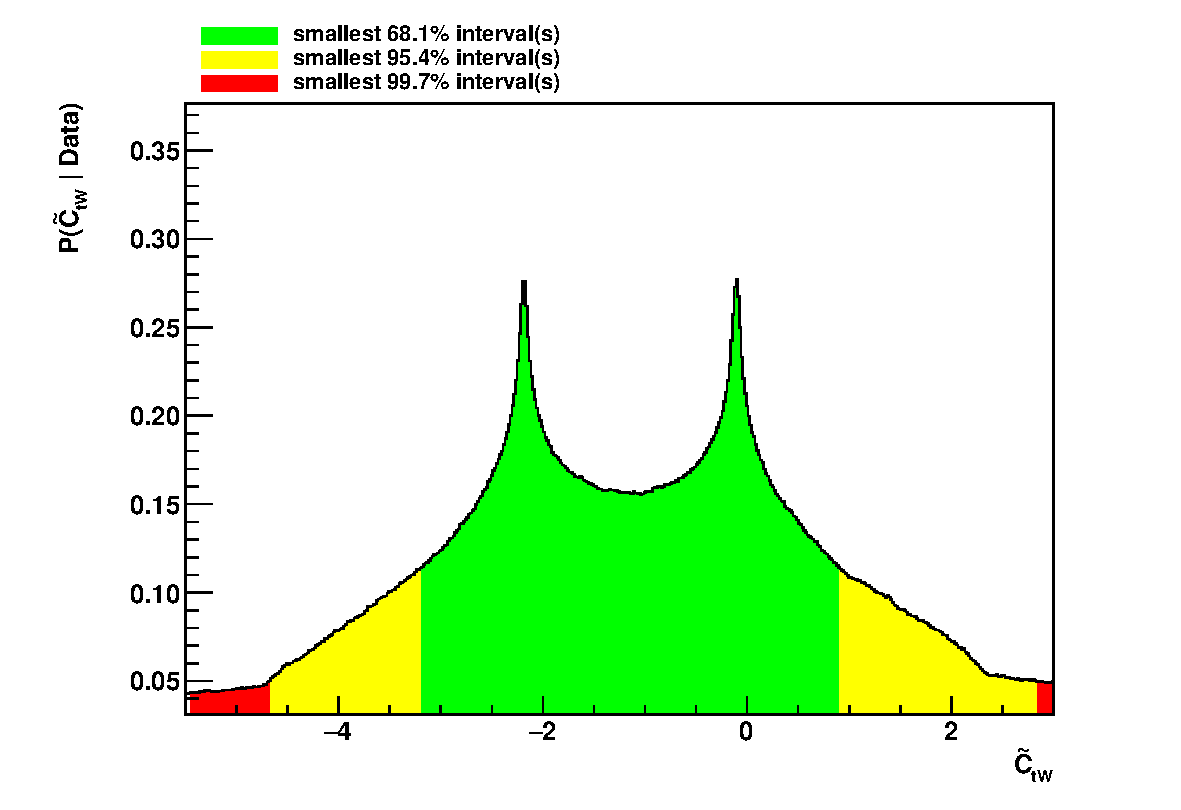
\includegraphics[width=0.8\textwidth]{Plots/ctw.pdf}
    \caption{Eindimensionale Posteriorverteilung des Wilson-Koeffizienten $\tilde{C}_{tW}$.}
    \label{fig:ctw}
\end{figure}
\begin{figure}
    \centering
    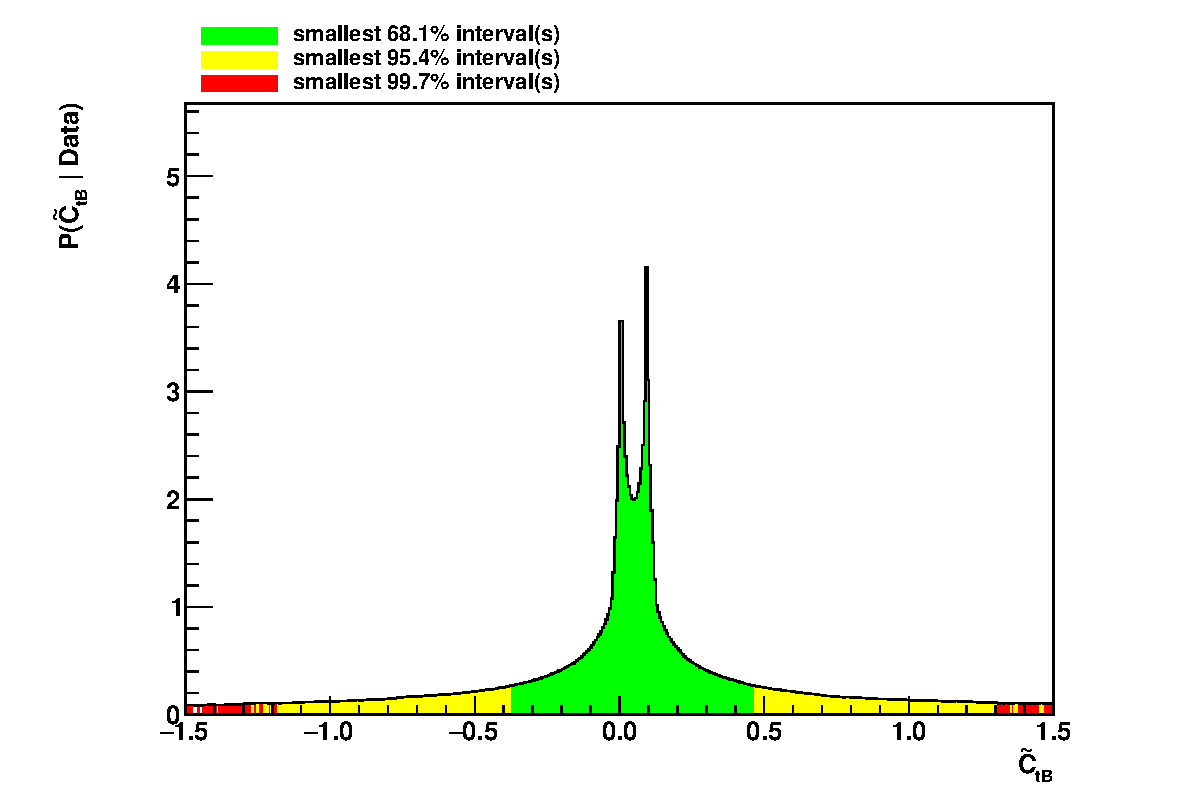
\includegraphics[width=0.8\textwidth]{Plots/ctb.pdf}
    \caption{Eindimensionale Posteriorverteilung des Wilson-Koeffizienten $\tilde{C}_{tB}$.}
    \label{fig:ctb}
\end{figure}
\begin{figure}
    \centering
    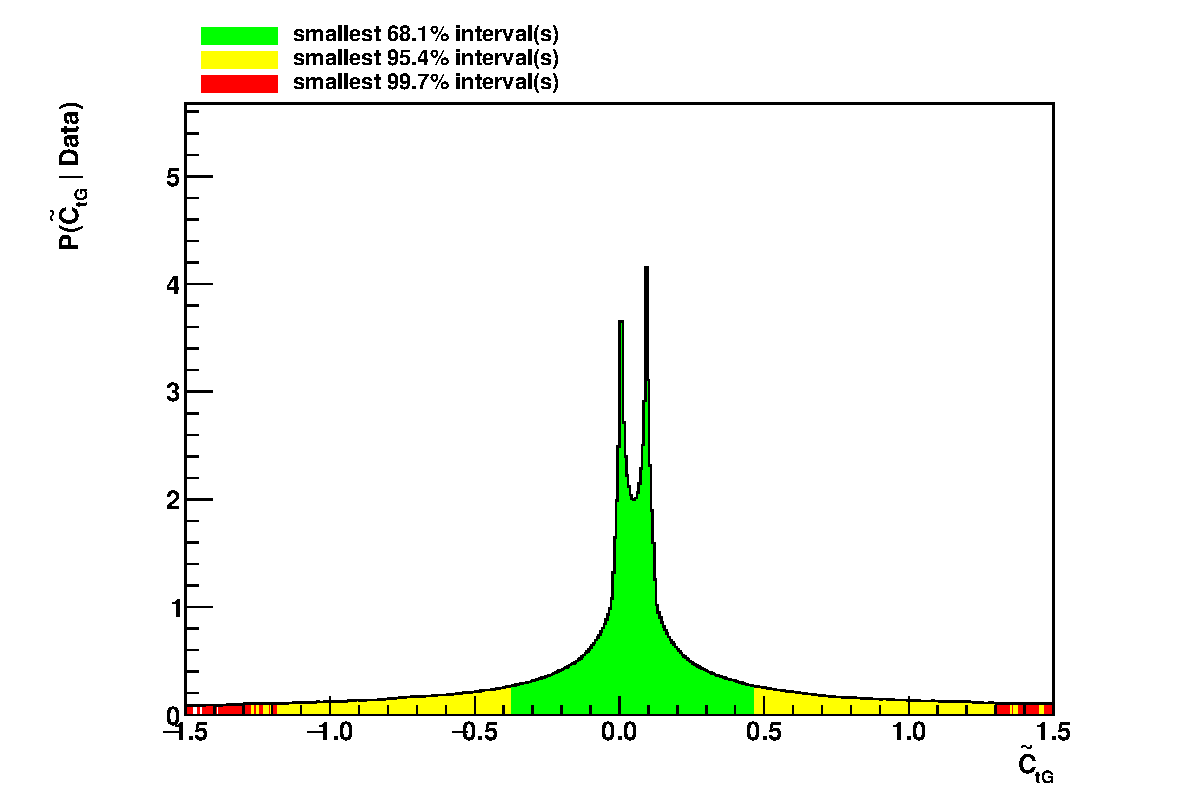
\includegraphics[width=0.8\textwidth]{Plots/ctg.pdf}
    \caption{Eindimensionale Posteriorverteilung des Wilson-Koeffizienten $\tilde{C}_{tG}$.}
    \label{fig:ctg}
\end{figure}
\begin{figure}
    \centering
    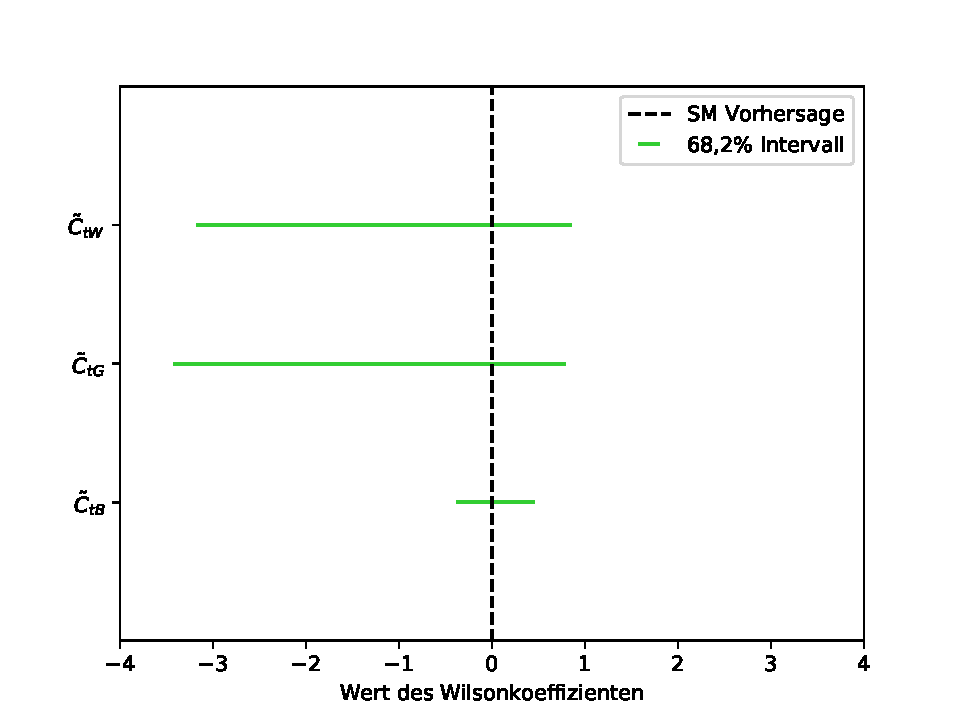
\includegraphics[width=0.7\textwidth]{Plots/wilson.pdf}
    \caption{Darstellung des kleinsten $\SI{68.1}{\percent}$ Intervalls der Wilson-Koeffizienten zur Veranschaulichung der Verträglichkeit mit Null.}
    \label{fig:wil}
\end{figure}
%
%
\chapter{Zusammenfassung}
Ein Bereich der aktueller Forschung in der Teilchenphysik liegt in der BSM-Physik, diese ist dadurch motiviert, dass verschiedene Effekte nicht mit dem Standardmodell zu erklären sind. Eine Möglichkeit diese Effekte zu beschreiben bieten modellunabhänigige effektive Feldtheorien. Ihr Vorteil ist, dass auch Teilchen, die an aktuellen Beschleunigern nicht produziert werden können, mit ihnen beschrieben werden können. Die Untersuchung des Top-Quarks im Zusammenhang von EFT ist dadurch motiviert, dass verschiedene Faktoren, wie beispielsweise die Yukawa-Kopplung des Top-Quarks, dafür sprechen, dass dieses stark an BSM-Physik koppeln könnte. \\
Im Rahmen dieser Arbeit erfolgte eine Interpretation von $t\bar{t}\gamma$-Messungen in Bezug auf EFT. Zunächst wurde eine Phasenraumstudie durchgeführt, um die in unterschiedlichen Phasenräumen durchgeführten ATLAS- und CMS-Messungen zu kombinieren. Dazu wurde ein Faktor zur Anpassung des CMS-Phasenraums an den ATLAS-Phasenraum bestimmt und auf die CMS-Messung angewandt. Die anschließende Kombination der Messungen, unter der Annahme, dass diese unkorreliert seien, lieferte:
\begin{align*}
  \sigma_{\text{Kombi}} = 150 \pm 18~ \si{\femto\barn}.
\end{align*}
Es fiel auf, dass das kombinierte Ergebnis sehr nah an dem ATLAS-Messwert lag. Daher lässt sich sagen, dass eine Kombination von Messungen nur sinnvoll ist, wenn sie im identischen oder nahezu gleichem Phasenraum durchgeführt wurden. Dies liegt vor allem an dem Einfluss der Unsicherheiten auf das Ergegnis einer Kombination. Im Anschluss erfolgte eine Korrelationsstudie, um den Einfluss einer möglichen Korrelation zwischen den Unsicherheiten der Messungen auf das Ergebnis der Kombination zu untersuchen. Dabei ergibt sich, dass die Kombination stark von einer möglichen Korrelation abhängt, sodass diese zunächst untersucht werden sollte.
Im zweiten Teil dieser Arbeit erfolgte die EFT-Interpretation des $t\bar{t}\gamma$-Produktionswirkungsquerschnitts mit dem EFT\textit{fitter}. Dafür wurden die Wilson-Koeffizienten $C_{tG}$, $C_{tW}$ und $C_{tB}$, der am Produktionswirkungsquerschnitt beteiligten Operatoren, untersucht. Innerhalb des kleinsten $\SI{68.1}{\percent}$-Intervalls sind alle drei Wilson-Koeffizienten mit Null verträglich. Die Intervalle der an der Photonabstrahlung beteiligten Wilson-Koeffizienten $C_{tW}$ und $C_{tB}$ sind jedoch relativ breit.\\
Dies motiviert eine Untersuchung dieser Wilson-Koeffizienten mit weiteren Messungen, wie beispielsweise des $t\bar{t}\gamma$-Produktionswirkungsquerschnitts, bei denen die entsprechenden EFT-Operatoren beteiligt sind. Dabei könnte sich eine Inkompatibilität mit Null ergeben und somit die Existenz der Operatoren $O_{tW}$ und $O_{tB}$ beweisen.


\appendix
% Hier beginnt der Anhang, nummeriert in lateinischen Buchstaben
\chapter{Anhang}
\begin{table}
  \centering
  \caption{Variation zur Wilson-Koeffizienten.}
  \begin{tabular}{lllll}
    \toprule
    $C_{tW}$ & $C_{tB}$ & $C_{tG}$ & $\sigma_{MC}$ & stat. Unsicherheiten\\
		\midrule
  0    &     0      &     0      &      682.9   &    0.85\\
  0    &     0      &     1      &      897.8   &    4.4\\
  0    &     0      &     -1     &      526.3   &    2.4\\
  0    &     0      &     10     &      576.3   &    26\\
  0    &     0      &     -10    &      1908    &    8.5\\
  0    &     0      &     20     &      17300   &    96\\
  0    &     0      &     -20    &      9434    &    82\\
  0    &     0      &     30     &      34890   &    140\\
  0    &     0      &     -30    &      23590   &    150\\
  0    &     1      &     0      &      686.7   &    2.7\\
  0    &     -1     &     0      &      679.4   &    3.2\\
  0    &     10     &     0      &      896.5   &    4\\
  0    &     -10    &     0      &      807.2   &    4.8\\
  0    &     20     &     0      &      1445    &    5.1\\
  0    &     -20    &     0      &      1266    &    5.7\\
  0    &     30     &     0      &      2326    &    8.6\\
  0    &     -30    &     0      &      2065    &    9.4\\
  1    &     0      &     0      &      690.8   &    3.4\\
  -1   &     0      &     0      &      678.8   &    3.5\\
  10   &     0      &     0      &      895.5   &    3.9\\
  -10  &     0      &     0      &      798.6   &    2.9\\
  20   &     0      &     0      &      1437    &    5.8\\
  -20  &     0      &     0      &      1261    &    4.9\\
  30   &     0      &     0      &      2324    &    7.6\\
  -30   &    0      &     0      &      2068   &     8.2\\
  \bottomrule
\end{tabular}
\label{tab:lit}
\end{table}
\begin{table}
  \centering
  \caption{Variation zur Wilson-Koeffizienten.}
  \begin{tabular}{lllll}
    \toprule
    $C_{tW}$ & $C_{tB}$ & $C_{tG}$ & $\sigma$ & stat. Unsicherheiten\\
		\midrule
  1     &    1      &     1      &      922.5  &     3.3\\
  -1    &    -1     &     -1     &      526.7  &     2.3\\
  1     &    1      &     -1     &      537.5  &     2.3\\
  -1    &     -1    &      1     &      893.1  &     4.7\\
  1     &     1     &      -1    &      530.7  &     2.1\\
  10    &    10     &     10     &      7032   &     55\\
  -10   &    -10    &     -10    &      3029   &     16\\
  -10   &     -10   &      10    &      5816   &     29\\
  10    &    10     &     -10    &      2213   &     15\\
  20    &    20     &     -20    &      10390  &     66\\
  -20   &    -20    &     20     &      17460  &     100\\
  20    &    20     &     20     &      21870  &     120\\
  -20   &    -20    &     -20    &      14210  &     100\\
  30    &    30     &     -30    &      25040  &     130\\
  -30   &    -30    &     30     &      36110  &     240\\
  30    &    30     &     30     &      45560  &     220\\
  -30   &    -30    &     -30    &      33320  &     160\\
  1     &    1      &     0      &      708.1  &     4.7\\
  -1    &    -1     &     0      &      675.7  &     2.7\\
  10    &    10     &     0      &      1443   &     5\\
  -10   &    -10    &     0      &      1263   &     8.2\\
  20    &    20     &     0      &      3539   &     15\\
  -20   &    -20    &     0      &      3173   &     12\\
  30    &    30     &     0      &      6979   &     25\\
  -30   &    -30    &     0      &      6446   &     22\\
    \bottomrule
  \end{tabular}
  \label{tab:lit}
\end{table}


\backmatter
\printbibliography[title=Literaturverzeichnis]


\chapter{Danksagung}

\cleardoublepage
\thispagestyle{empty}
\section*{Eidesstattliche Versicherung}
Ich versichere hiermit an Eides statt, dass ich die vorliegende Abschlussarbeit mit dem Titel \enquote{\thetitle} selbstständig und ohne unzulässige fremde Hilfe erbracht habe.
Ich habe keine anderen als die angegebenen Quellen und Hilfsmittel benutzt, sowie wörtliche und sinngemäße Zitate kenntlich gemacht. 
Die Arbeit hat in gleicher oder ähnlicher Form noch keiner Prüfungsbehörde vorgelegen.

\vspace*{1cm}\noindent
\begin{center}
  \begin{tabular}{@{}p{0.4\textwidth}@{\hspace{0.15\textwidth}}p{0.4\textwidth}@{}}
  \rule{\linewidth}{0.25pt}& \rule{\linewidth}{0.25pt}\\
  Ort, Datum & Unterschrift
  \end{tabular}
\end{center}

\subsection*{Belehrung}
Wer vorsätzlich gegen eine die Täuschung über Prüfungsleistungen betreffende Regelung einer Hochschulprüfungsordnung verstößt, handelt ordnungswidrig.
Die Ordnungswidrigkeit kann mit einer Geldbuße von bis zu \SI[round-mode=places, round-precision=2]{50000}{€} geahndet werden. 
Zuständige Verwaltungsbehörde für die Verfolgung und Ahndung von Ordnungswidrigkeiten ist der Kanzler/die Kanzlerin der Technischen Universität Dortmund. 
Im Falle eines mehrfachen oder sonstigen schwerwiegenden Täuschungsversuches kann der Prüfling zudem exmatrikuliert werden \mbox{(\S\,63 Abs. 5 Hochschulgesetz --HG--).}

Die Abgabe einer falschen Versicherung an Eides statt wird mit Freiheitsstrafe bis zu 3 Jahren oder mit Geldstrafe bestraft.

Die Technische Universität Dortmund wird ggf.\ elektronische Vergleichswerkzeuge (wie z.\,B.\ die Software \enquote{turnitin}) zur Überprüfung von Ordnungswidrigkeiten in Prüfungsverfahren nutzen. \\[\baselineskip]

\noindent Die oben stehende Belehrung habe ich zur Kenntnis genommen.\\[1cm]
\begin{center}
\begin{tabular}{@{}p{0.4\textwidth}@{\hspace{0.15\textwidth}}p{0.4\textwidth}@{}}
\rule{\linewidth}{0.25pt}& \rule{\linewidth}{0.25pt}\\
Ort, Datum & Unterschrift
\end{tabular}
\end{center}

\end{document}
